\chapter{Pruebas y resultados} \label{chap:test_results}

Este apartado, refiere a las pruebas realizadas al sistema PARKIBIP, conformado por la aplicación móvil y ambos dispositivos IMU. 

Por un lado pruebas estáticas, exploratorias, funcionales y para-funcionales. El propósito fue aumentar la confiabilidad del mismo a través de su evaluación de calidad; mediante abordajes que verifiquen la legibilidad del código, la escalabilidad del sistema, la correcta interoperabilidad entre componentes y, sobre todo, la detección temprana de incidentes que puedan generar una falla posterior (e.g. omitir eventos de desconexión de los IMU, ocasiona el quiebre de la aplicación).

Por otro lado, se evaluó a PARKIBIP en funcionamiento a través de pruebas de usabilidad y eficiencia. El objetivo de estas pruebas es comparar la performance del algoritmo final -resultado de la combinación de métodos- frente a datos conocidos, y estudiar en qué casos particulares el algoritmo tiene comportamientos diferentes (e.g. en términos de error relativo y tiempos de ejecución)

\section{Pruebas Estáticas: Peer Code Review}

En primer lugar, se empleó durante todo el proceso de desarrollo una técnica de verificación estática, denominada revisión de código por pares (del inglés, Peer Code Review). Esta práctica sistemática de desarrollo consiste en chequear manualmente el código y sus cambios de a pares, a fín de  encontrar problemas, errores y vulnerabilidades, tan pronto como sea posible. Al ser una verificación estática, se realiza sobre el código sin ejecutarlo. 
\noindent Acorde con la herramienta Gitlab, empleada en PARKIBIP para gestionar el repositorio y controlar el versionado de código (ver \nameref{project:version-control}), fue de gran utilidad su herramienta integrada de revisión de código ligero. El procedimiento establecido fue, con cada modificación de código eventualmente finalizada, se le solicita al otro miembro del equipo la inclusión de dichos cambios, mediante el comando \textit{Pull Request}. Luego, el revisor asignado y orientado a las oportunidades de mejora y a la crítica constructiva; comienza a verificar el cumplimiento de los estándares de codificación, identificar posibles errores en el código fuente, detectar posibles problemas de diseño en la nueva solución. La herramienta, habilita a realizar comentarios línea a linea del código, obtener una vista previa de los cambios en comparación con el código vigente del repositorio -para ver qué se está proponiendo-, mantener una discusión activa del código, entre otras cosas. A efectos de comprender lo antedicho, se propone la figura Fig. \ref{FIG:pr-review} como ejemplo de revisión. En la misma, se puede visualizar con color verde las nuevas modificaciones y con rojo las eliminaciones de código, además de un comentario del revisor asignado.

\begin{figure}[H]
\centering
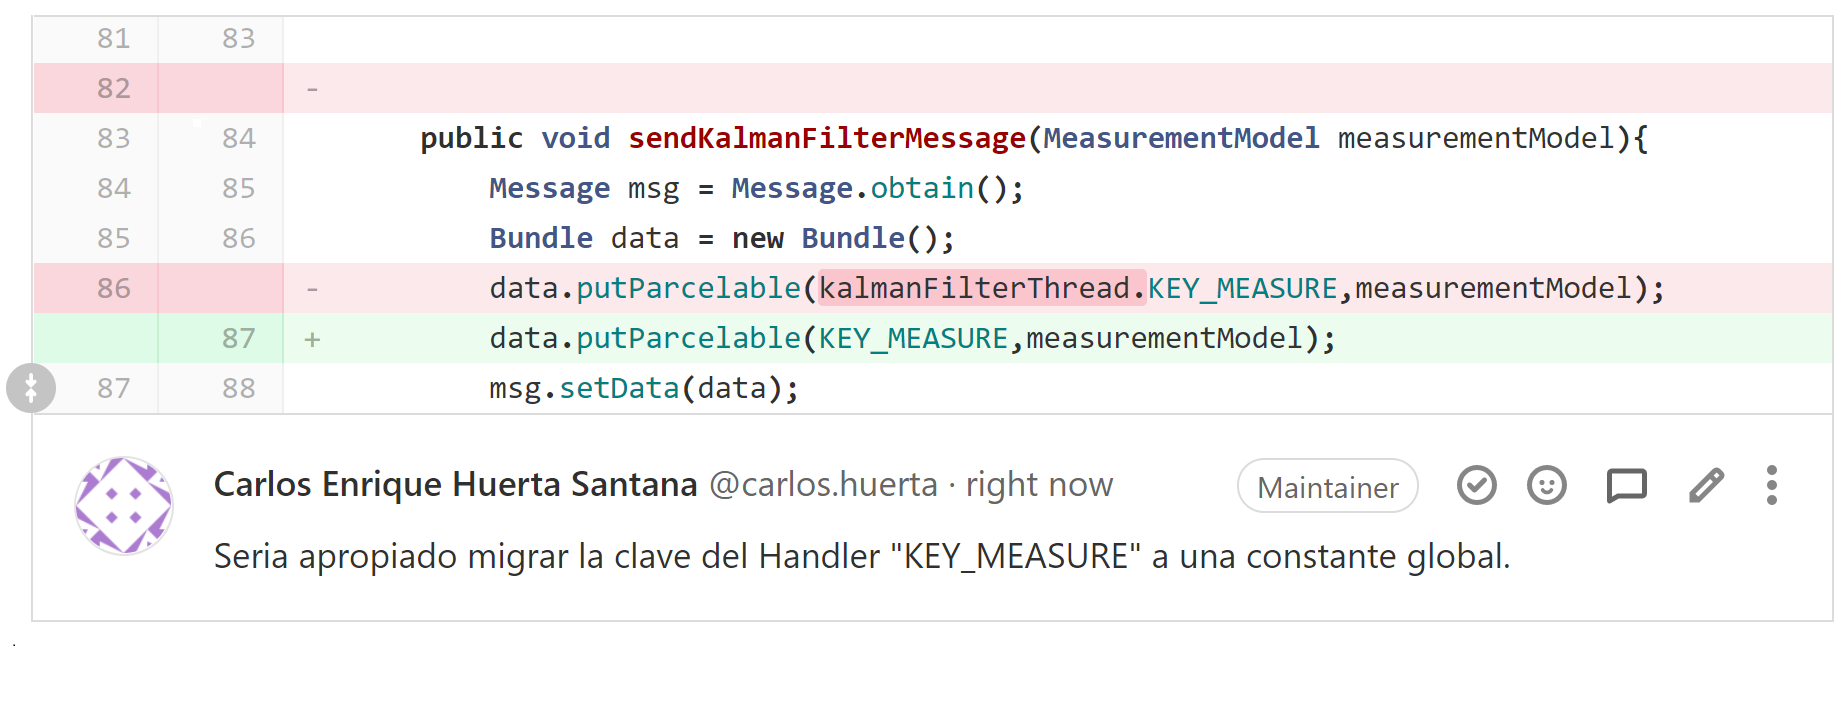
\includegraphics[width=\textwidth]{TESIS/imagenes/chap06/pr-comments.PNG}
\caption{Ejemplo de revisión de código entre pares sobre la petición de modificación hacia la rama principal de desarrollo -\textit{pull request}-. Con color verde se visualizan las nuevos cambios y con rojo las eliminaciones de código, además de un comentario del revisor asignado. }
\label{FIG:pr-review}
\end{figure}

\noindent De forma adicional, la figura Fig. \ref{FIG:pr-result}, muestra un resultado de un proceso de verificación y validación estática con la estrategia \textit{Code Review} con la herramienta GitLab. Se observa la aprobación y posterior mezclado de código por parte del revisor bajo el indicador \textit{Merged}, la cantidad y descripción de cambios incluidos, así como también el origen y el destino de los cambios.

\begin{figure}[H]
\centering
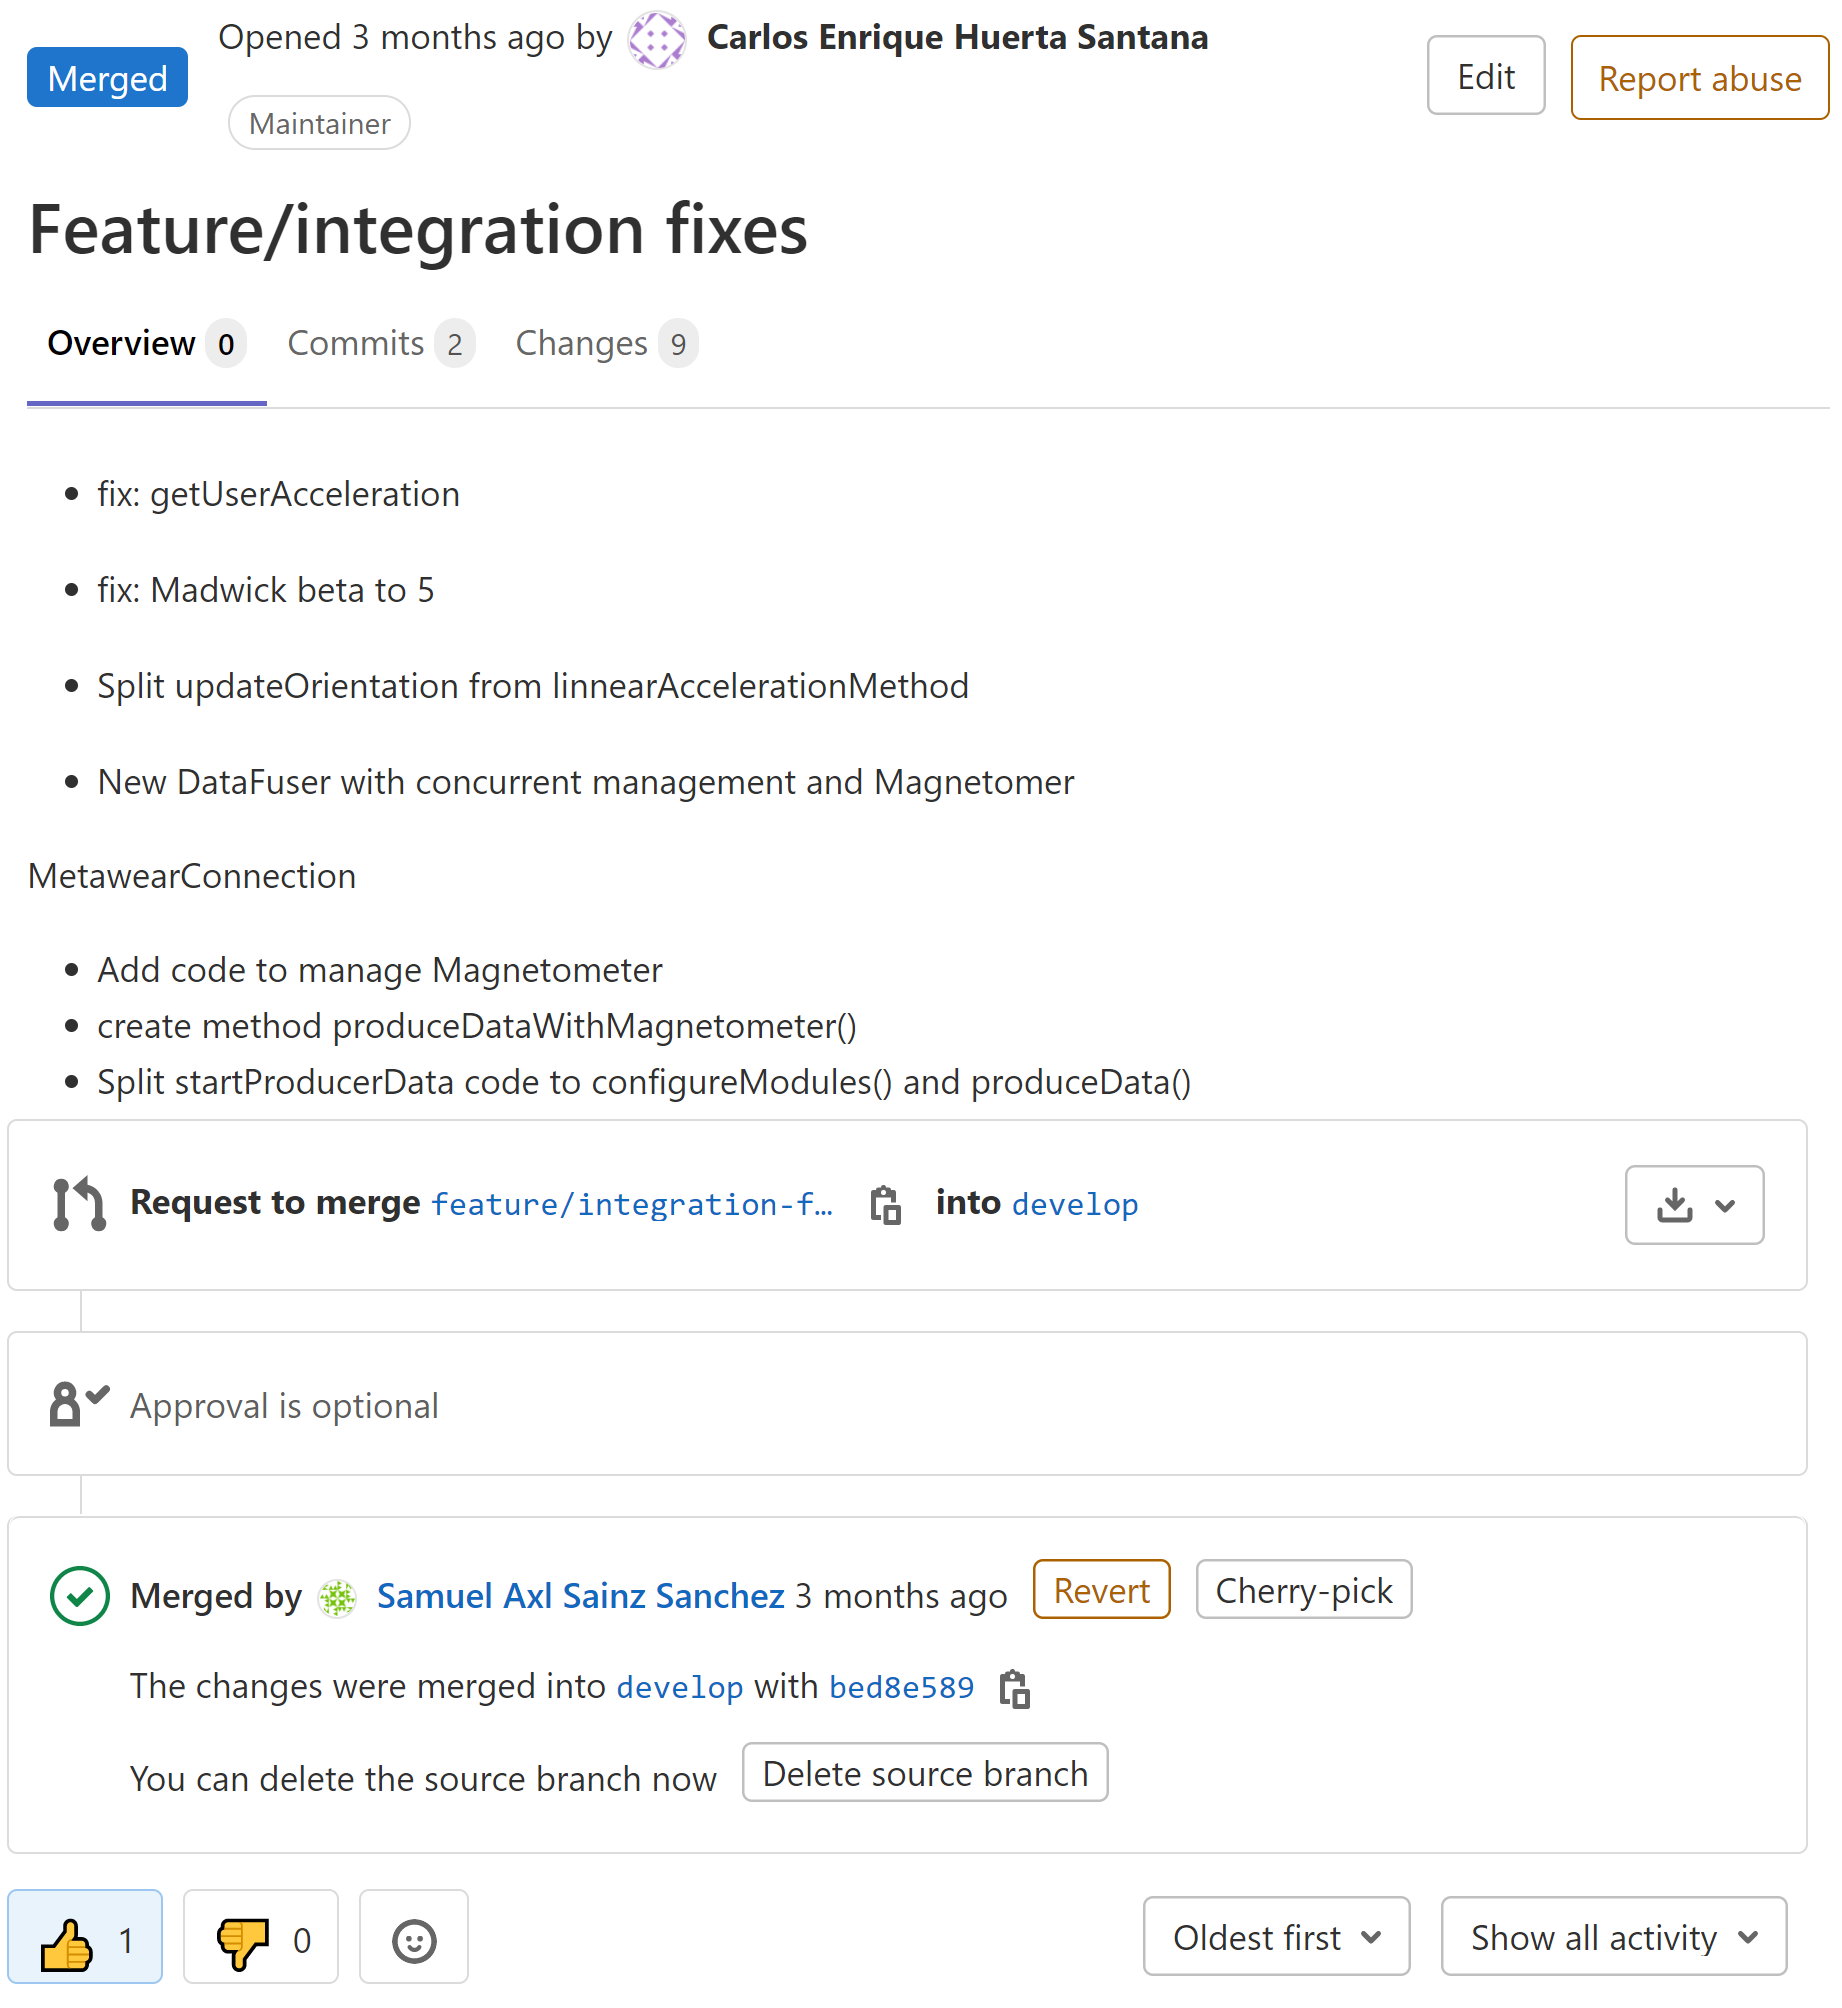
\includegraphics[width=\textwidth]{TESIS/imagenes/chap06/pr.PNG}
\caption{Resultado de un proceso de verificación y validación estática con la estrategia \textit{Code Review} en la herramienta GitLab}
\label{FIG:pr-result}
\end{figure}

\section{Pruebas funcionales: Unitarias e Integración}

%TIPO DE PRUEBAS
Por otro lado, para realizar las pruebas funcionales, se siguió una estrategia de Testing Planificado, a partir del diseño de casos de prueba y su posterior ejecución. Según la etapa particular del proceso de desarrollo, fueron implementadas diferentes pruebas:

\begin{itemize}
    \item Pruebas Unitarias: Las pruebas unitarias tienen por objetivo aislar cada componente individual del sistema, luego de su desarrollo, y demostrar que su funcionalidad y estructura es correcta.
    \item Pruebas de Integración: Las pruebas de integración tienen como propósito verificar la correcta interoperabilidad entre los distintos componentes del sistema, una vez que han sido probados mediante las pruebas unitarias. La idea por detrás, es comprobar que dichos componentes interactúan correctamente a través de sus interfaces, tanto internas como externas, cubren la funcionalidad establecida y se ajustan a los requisitos no funcionales
\end{itemize}

%FRAMEWORK
Así, el objetivo de esta actividad fue detectar defectos, problemas o anomalías, inyectadas en en el software PARKIBIP ya sea por omisión o por error. Para llevar a cabo esta tarea, se utilizó el entorno de trabajo (en inglés, framework) JUnit para Android, versión 4.12. JUnit brinda un marco de ejecución para las pruebas, corre fácilmente los conjuntos de prueba definidos, presenta una API que facilitan la comparación y el manejo de errores, y el armado de cada prueba. 
%Anotaciones de Test
Por consiguiente, se desarrolló en el lenguaje Android los llamados \textit{Test Suites}, representando un conjunto de pruebas relacionadas que comparten el mismo \textit{Fixture} (i.e. pre-condiciones o estado necesario para la prueba). Dichas pruebas del \textit{Test Suite} son independientes y representadas mediante una clase, bajo la anotación \textit{@Test} para indicar que es una prueba. La modalidad utilizada al probar fue la de caja negra, en la cual se comprueba el correcto funcionamiento de los componentes, analizando únicamente las entradas/salidas y verificando que el resultado es el esperado. Para ello, las anotaciones de JUnit utilizadas fueron:
\begin{itemize}
    \item \textit{@Suite}: Esta anotación permite agrupar algunos casos de prueba unitarios y ejecutarlos juntos
    \item \textit{@Test}: Etiqueta un método para que sea considerado como caso de prueba
    \item \textit{@Before}: Indica que un método particular se ejecuta previo a la prueba. En general, se emplea para inicializar el contexto del test (e.g. probar el filtro de Kalman requiere conocer previamente la orientación dada por al filtro de Orientación) 
    \item \textit{@After}: Indica que un método particular se ejecuta luego de una prueba. En caso de asignarse recursos con la anotación @Before, este método permite liberarlos después de que se ejecute la prueba (i.e. libera el contexto)
    \item \textit{assert}: Función que verifica el comportamiento o estado de la unidad bajo prueba
\end{itemize}

%Tests y suite principales
\noindent Con el propósito de ejemplificar y presentar los casos de prueba esenciales en PARKIBIP, se sintetizan algunas \textit{Suites}  que encapsulan ciertas pruebas -por convención, todas las clases de prueba finalizan con la palabra ``Test''-:
\begin{itemize}
    \item \textit{Quaternion.suite}: Contiene el conjunto de casos de prueba relacionados a la representación de la orientación en el formato de quaterion. Las clases desarrolladas fueron las siguientes:
    \begin{itemize}
        \item \textit{CalibrationQuaternionTest}. Con la anotación \textit{@Before}, se define el conjunto de observaciones de prueba - tomadas de un archivo auxiliar- y el valor esperado del quaternion para dichas mediciones. Luego, se ejecuta la prueba comenzando por la estandarización al \gls{SI}. Se recorren 20 mediciones, aplicando la función de calibración -perteneciente a la librería de algoritmos implementados, desde ahora APIAlgorithm-. Finalmente, se compara el resultado esperado frente cada una de las 4 componentes del vector quaternion obtenido, con el comando de igualdad \textit{assertEquals}
        \item \textit{QuaternionToRotationMatrixTest}. Dados un quaternion y la matriz de rotacion -conocidos-, definidos en \textit{@Before}, se corre la prueba invocando la función \textit{ConvertToRotationMatrix()} de la \textit{APIAlgorithm}. Las entradas de la matriz obtenida y esperada son evaluadas una a una con \textit{assertEquals}.
        \item \textit{QuaternionToEulerAngleTest}. Procedimiento análogo a \textit{QuaternionToRotationMatrixTest}, con la distincion que, en vez de una matriz es un vector.
        \item \textit{QuaternionToConjugateTest}. Similar a los casos previos,  dados un quaternion y su conjugado -conocidos-, establecidos en \textit{@Before}, se ejecuta la prueba invocando la función \textit{ConvertToConjugate()} de la \textit{APIAlgorithm}. Luego, las entradas de los vectores de quaternions conjugados son comparadas mediante \textit{assertEquals}.
        \item \textit{QuaternionTestSuite}. Mediante su definición, le permite al entorno de desarrollo identificar y correr todas las pruebas pertenecientes al módulo o \textit{Suite}
    \end{itemize}
    \item \textit{Orientation.suite}:Contiene el conjunto de casos de prueba relacionados al calculo de la orientación mediante el filtro de orientación en \ref{FIG:madgwick}. Las clases desarrolladas fueron:
    \begin{itemize}
        \item \textit{UpdateOrientationTest}. Dado el quaternion esperado, que representa la orientación del sensor relativa al marco Tierra, y un conjunto de $21$ mediciones, ambos definidos en \textit{@Before}. Se recorren 20 mediciones, aplicando la función de calibración \textit{calibrateQuaternion} de la \textit{APIAlgorithm}, se inicializa el filtro de orientación para dicho quaternion, y luego se actualiza el filtro de orientación con la ultima medición, \textit{updateOrientation(measure)}. Finalmente, se comparan las componentes de los vectores esperado y obtenido.
        \item \textit{OrientationTestSuite}. Mediante su definición, le permite al entorno de desarrollo identificar y correr todas las pruebas pertenecientes a la \textit{Suite}.
    \end{itemize}
    \item \textit{ZeroVelocityDetector.suite}: Todas las pruebas asociadas al calculo de momentos de cero velocidad. Las clases desarrolladas fueron:
    \begin{itemize}
        \item MVZeroVelocityDetectorTest: Primero, el test establece  el algoritmo de detección de velocidad cero \textit{MovingVarianceDetector}, bajo el soporte del controlador de configuraciones PARKIBIP \textit{ConfigurationProvider}. Luego, el test almacena en memoria el conjunto de valores de cero velocidad de prueba -valores esperados- y el conjunto de mediciones de prueba - tomadas de un archivo auxiliar- (todo en \textit{@Before}). Se ejecuta el test iterando sobre las mediciones y llamando a la función \textit{zeroVelocityDetector.update(measure)} del detector particular. Para concluir, itera cada resultado y los compara contra su correspondiente valor esperado.
        \item GlrtZeroVelocityDetectorTest. Idéntico al caso previo, con la salvedad que el detector elegido es \textit{GLRTDetector}.
        \item \textit{ZeroVelocityDetectorTestSuite}. Mediante su definición, le permite al entorno de desarrollo identificar y correr todas las pruebas pertenecientes a la \textit{Suite} \textit{ZeroVelocityDetector}
    \end{itemize}
    \item \textit{KalmanFilter.suite}: Modulo de prueba complejo, combina diversos algoritmos para construir el vector de estados de Kalman. Las clases desarrolladas fueron:
    \begin{itemize}
        \item \textit{KalmanFilterAlgorithmTest}. El caso de prueba emplea un conjunto de mediciones inerciales de acceso libre, cuyo resultado velocidad promedio es conocido. Así, bajo la anotación \textit{@Before}, el test levanta las mediciones en memoria -tomadas de un archivo auxiliar-, y establece: (i) el algoritmo GLRT -como algoritmo de cero velocidad-, (ii) el resultado esperado, (iii) un valor $\theta$, como la desviación aceptable para la estimación, (iv) valores de frecuencias a utilizar. Luego, inicia la ejecución del test. Primero, calibra la orientación inicial del dispositivo, después,  itera sobre cada medición del conjunto de datos realizando los pasos:
        \begin{itemize}
            \item Ejecuta la función \textit{z = zeroVelocityDetector.update(measure)} del detector, para identificar momentos de cero velocidad en una ventana de tiempo
            \item Actualiza el quaternion del filtro de Orientación, bajo el método \textit{updateOrientation(measure)}
            \item Ejecuta el filtro de Kalman llamando a la función \textit{state = kalmanFilterZupdt.runFilter(measure,z)}
            \item Cada vector de estado obtenido es puesto en una estructura de almacenamiento en memoria
        \end{itemize}
        Finalmente, calcula la velocidad promedio como la sumatoria de normas de las velocidades instantáneas tridimensionales sobre la cardinalidad del conjunto, para luego comparar la velocidad media esperada con la obtenida. Se utiliza el comando \textit{assertEquals} con el valor $\theta$, que indica la diferencia máxima entre las medidas para que el caso sea satisfactorio.
        \item \textit{KalmanFilterAlgorithmAUPTest}. \textbf{Este caso de test es esencial para la aplicación, ya que integra y combina todos los módulos necesarios para el funcionamiento de PARKIBIP en productivo. Es decir, emplea datos reales de PARKIBIP a partir de experimentos en la Asociación Uruguaya de Parkinson (AUP), y el flujo de comunicación entre los componentes finales.} Su ejecución es análoga al caso previo, con la salvedad en los datos de prueba y frecuencias empleadas.
        \item \textit{KalmanFilterTestSuite}. Mediante su definición, le permite al entorno de desarrollo identificar y correr todas las pruebas pertenecientes a la \textit{Suite}.
    \end{itemize}
\end{itemize}


\noindent Viendo el flujo de realización de pruebas, se puede apreciar la aplicación de una estrategia  de integración ascendente (del inglés, Bottom-Up). Es decir, se construyen primero los componentes menos dependientes y luego se van integrando para construir otros de mayor jerarquía. Para el caso, primero lo vinculado a Quaternions y  el filtro de orientación, siguiendo por los detectores de velocidad cero, para finalizar con el filtro de Kalman.

%Diseño de casos de prueba
Por otra parte, con el propósito de complementar las actividades del proceso de pruebas funcionales, el apéndice \nameref{apendice:tests-cases} describe los 70 casos diseñados y ejecutados, a través de una matriz de casos de prueba. Cada uno incluyendo un identificador, su escenario, caso de test, pre-condiciones, prioridad, etapa, resultado esperado, entre otros.  

%Coverage

\section{Prueba funcional: Filtro de Orientación PARKIBIP}

A efectos de probar adecuadamente el filtro de Orientación, con datos reales, provenientes del IMU de PARKIBIP; se desarrolló una aplicación gráfica de escritorio, a modo de prueba de concepto (siglas en inglés, PoC, Proof of Concept). Esta, PoC se encarga de rotar un cubo 3D en tiempo real, según las mediciones que va recopilando del IMU conectado.

De esta manera, se desarrolló en el lenguaje \gls{.NET}, un sistema Cliente y Servidor. El Servidor, integrado a un IMU, recopila los datos inerciales -acelerómetro, giroscopio, magnetómetro-, y se los envía a el Cliente. Al recibir los datos, el Cliente, ejecuta el filtro de Orientación obteniendo en cada instante un quaternion. A su vez, el Cliente presenta una interfaz gráfica con un cubo en 3 dimensiones. Cuando el Cliente finaliza el cálculo de un quaternion, dispara un evento con dicho resultado que desencadena la rotación del cubo según los valores estimados. 

Entonces, la funcionalidad de la PoC, es emular en 3D y en tiempo real, la misma orientación que el dispositivo IMU, como si fuera un espejo. Así, es fácil corroborar la correctitud del cómputo de la orientación observando las semejanzas del IMU y del cubo. Las sub-figuras de la figura Fig. \ref{fig:3d rotation-orientation}, emulan en tiempo real las rotaciones del IMU mediante el cubo 3D. Además, se adjunta una grabación -video- circular de este proceso \footnote{Las grabaciones circulares se encuentran disponibles en el sitio  \href{https://drive.google.com/drive/folders/1qmg-Nex1i13uaCr66KOUZ3LE5vgFuK2W?usp=sharing}{PARKIBIP-grabaciones-circulares}
}.

\begin{figure}[!h]
     \centering
     \begin{subfigure}[b]{0.4\textwidth}
         \centering
         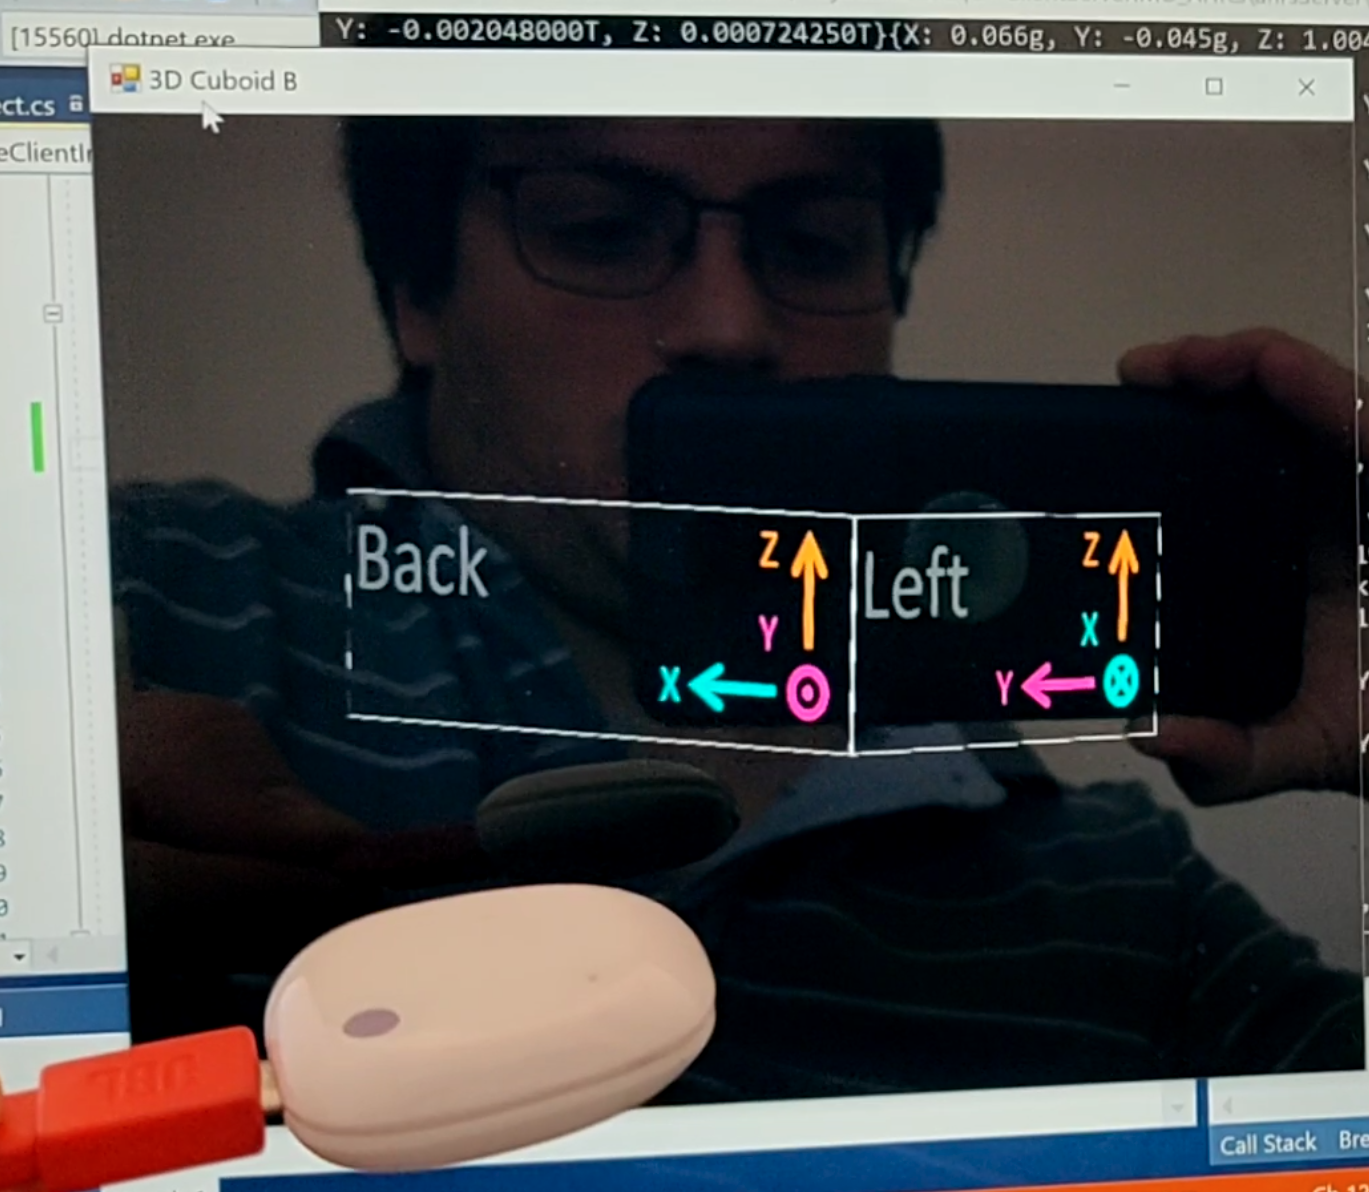
\includegraphics[width=4cm]{TESIS/imagenes/chap06/regular-orientation.png}
         \caption{Orientación regular del IMU-Cubo3D en el marco terrestre. }
     \end{subfigure}
     \begin{subfigure}[b]{0.4\textwidth}
         \centering
         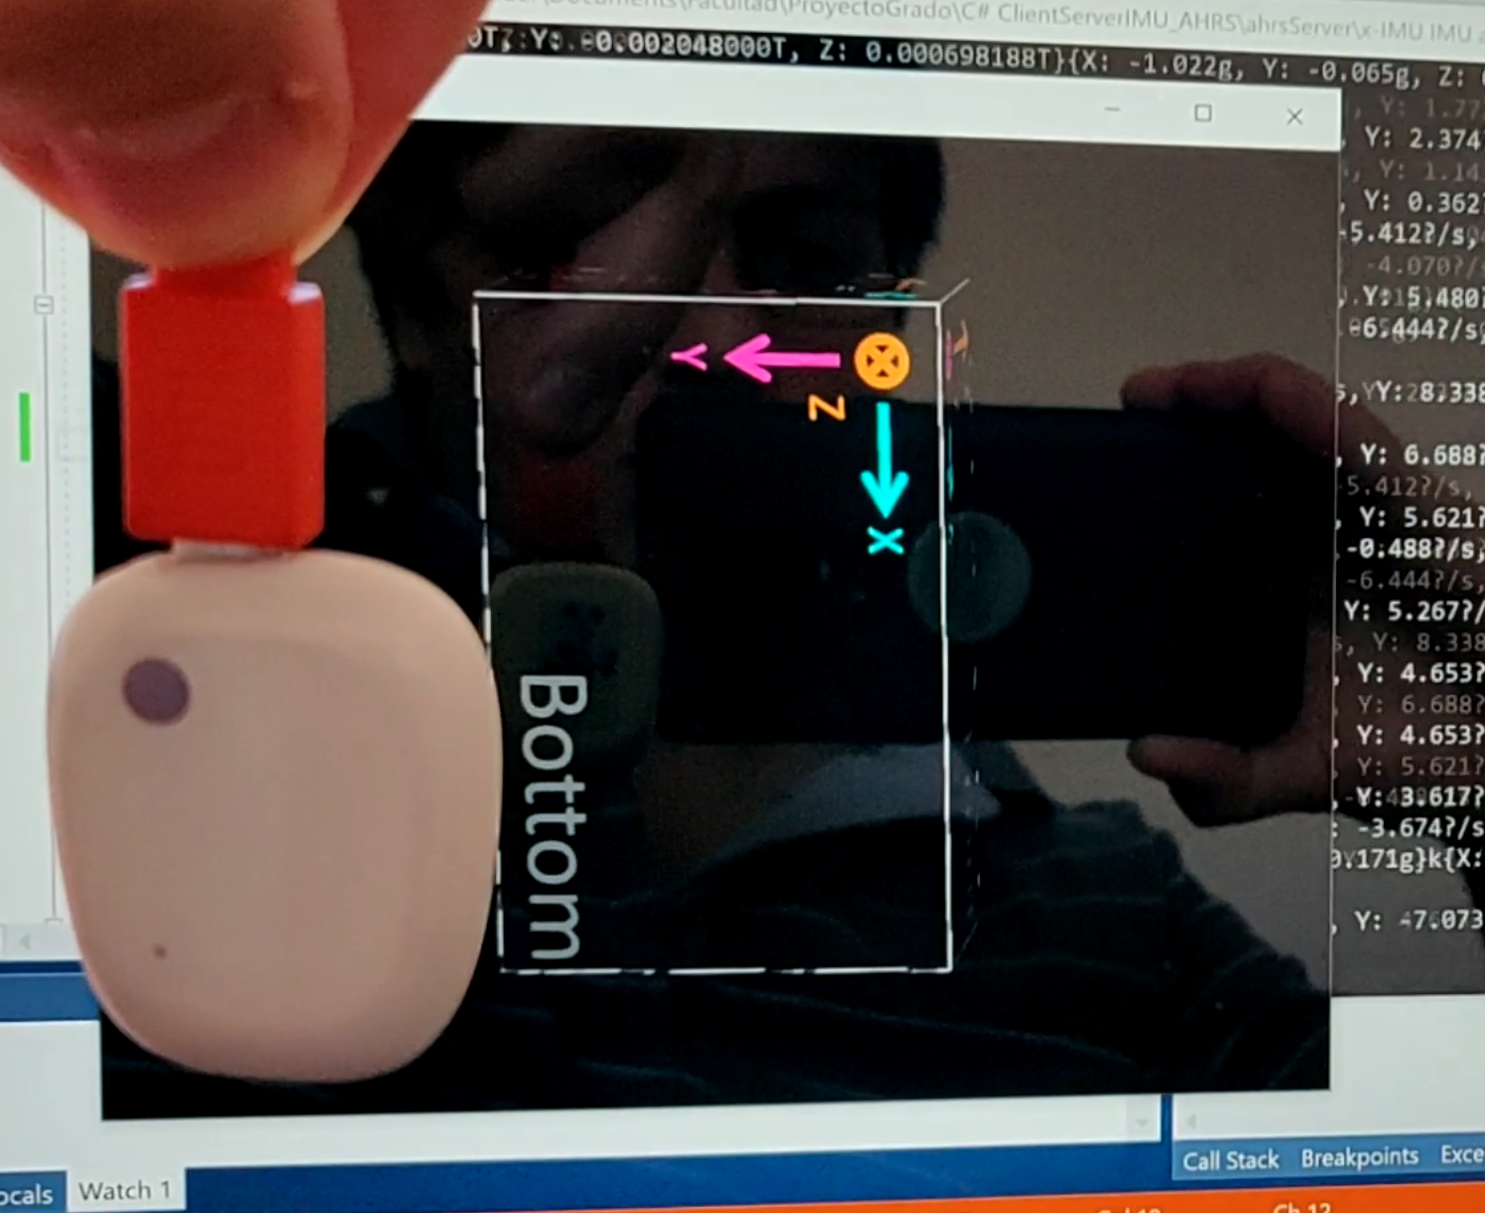
\includegraphics[width=4cm]{TESIS/imagenes/chap06/top-orientation.png}
    \caption{Orientación inferior del IMU-Cubo3D en el marco terrestre.}
     \end{subfigure}
      \begin{subfigure}[b]{0.4\textwidth}
         \centering
         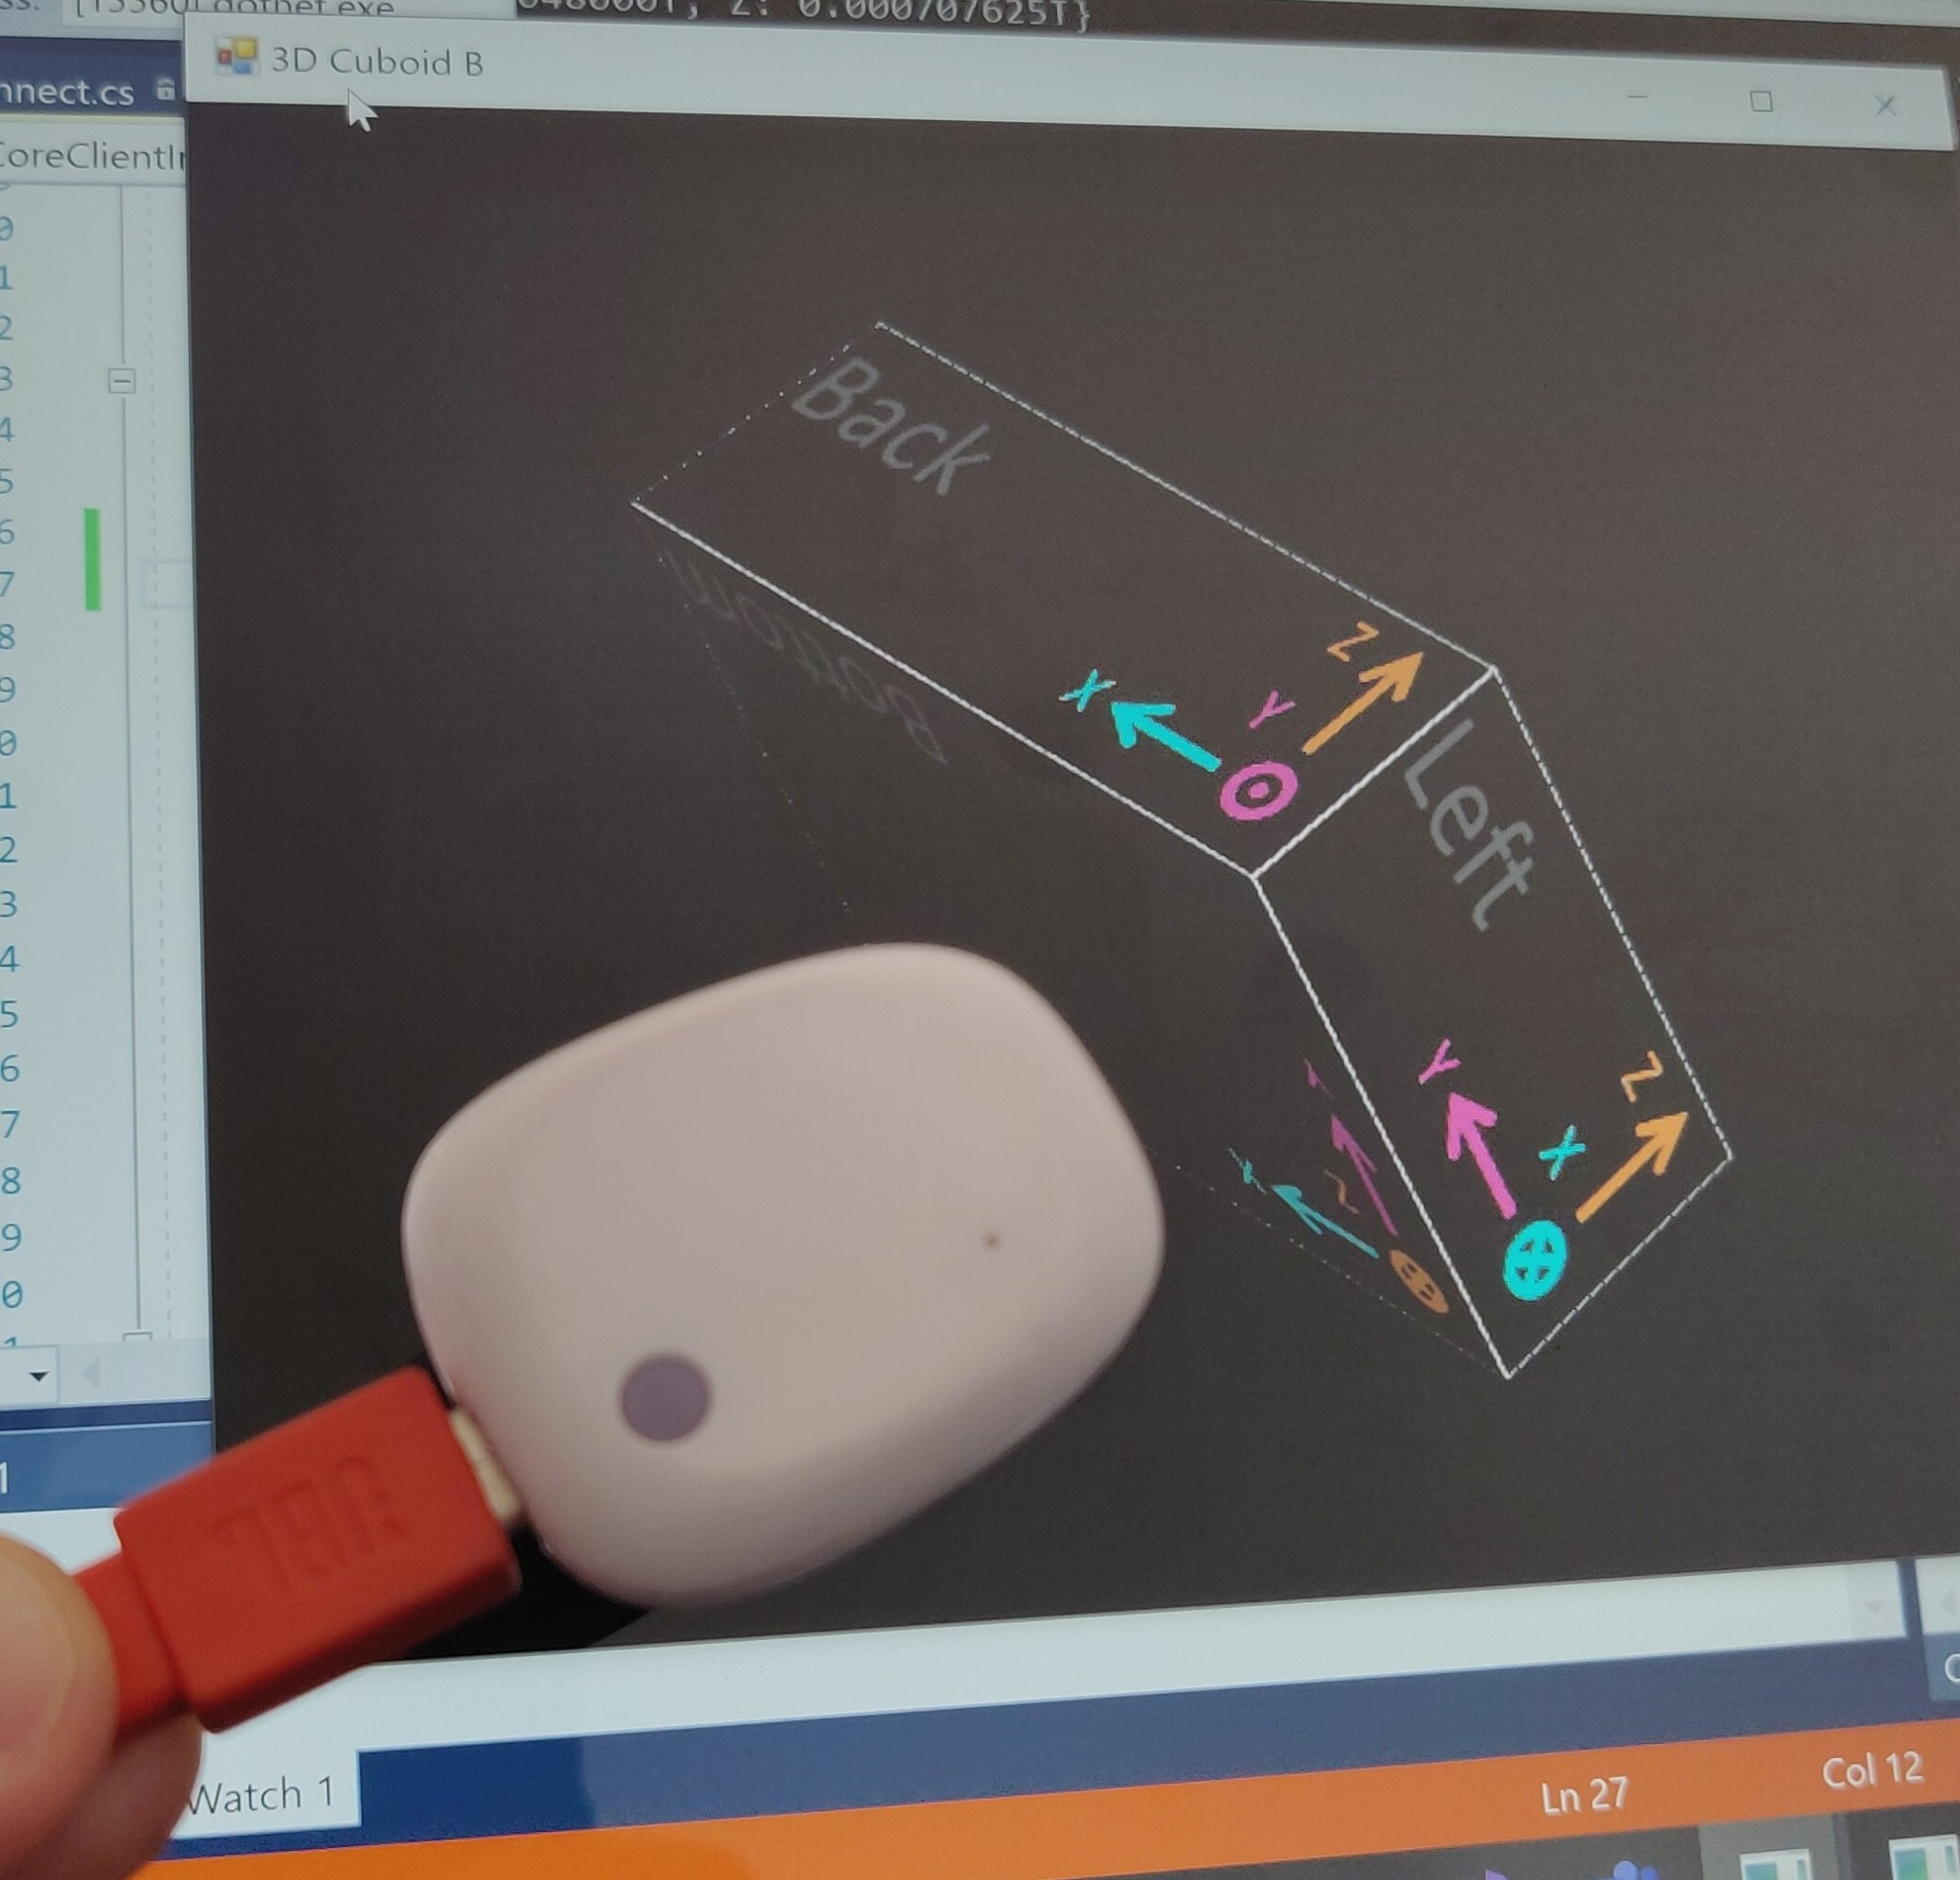
\includegraphics[width=4cm]{TESIS/imagenes/chap06/inclined-orientation.jpg}
    \caption{Orientación inclinada del IMU-Cubo3D en el marco terrestre.}
     \end{subfigure}
      \begin{subfigure}[b]{0.4\textwidth}
         \centering
         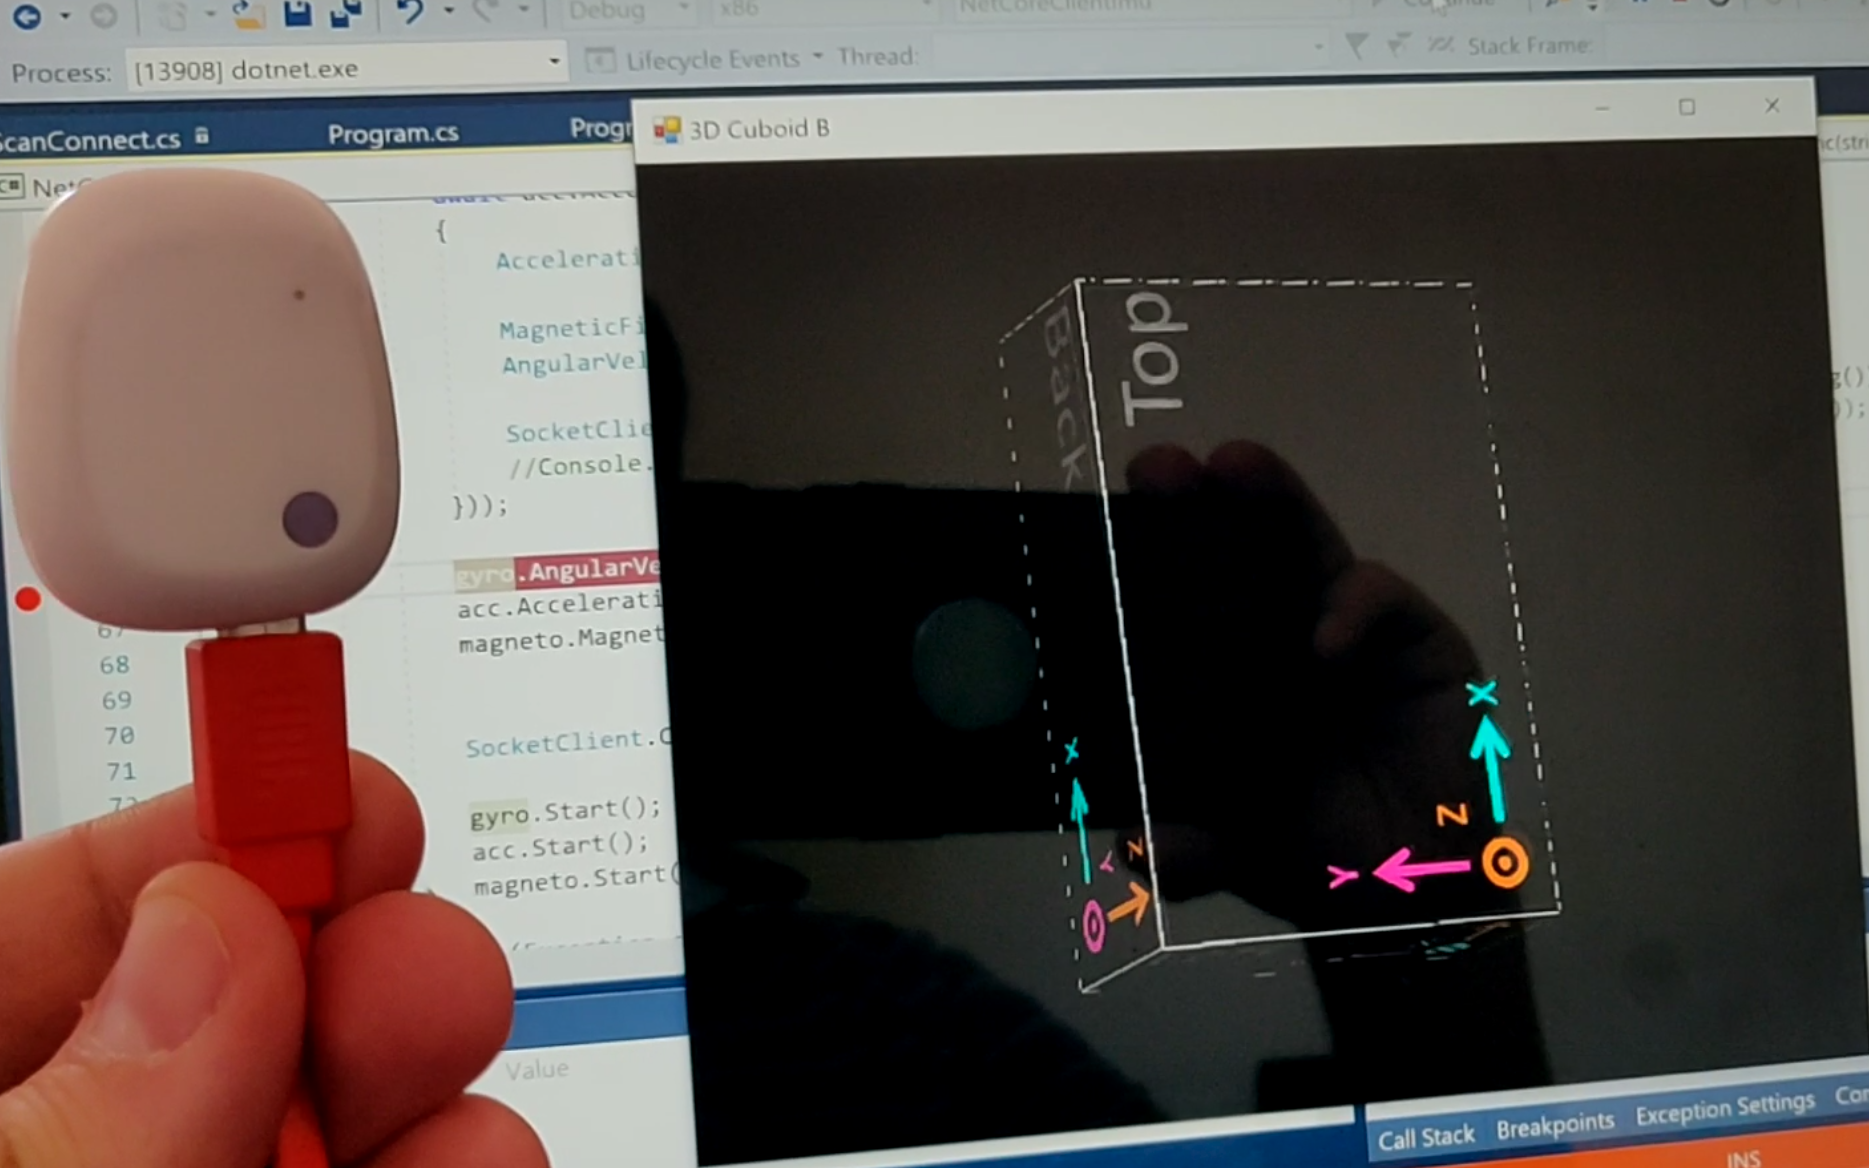
\includegraphics[width=6cm]{TESIS/imagenes/chap06/bottom-orientation.png}
         \caption{Orientación superior del IMU-Cubo3D en el marco terrestre.}
     \end{subfigure}
     \caption{Demostración gráfica de la orientación del IMU en tiempo real utilizando un cubo 3D mediante aplicación de escritorio .NET}
     \label{fig:3d rotation-orientation}
 \end{figure}

Debido a las complejidades numéricas de PARKIBIP, dicha PoC se propuso con la idea de:

\begin{itemize}
    \item Facilitar las pruebas en un entorno de desarrollo mas simple,  ágil y sin la necesidad de un teléfono inteligente
    \item Probar diversas frecuencias y configuraciones sobre el IMU que impacten en la orientación.
    \item Probar el método de consolidación de datos o Data Fuser
    \item Identificar y solucionar un error ``indescifrable'' por los integrantes del proyecto en la aplicación móvil Android. El error fue detectado al graficar en tiempo real la velocidad instantánea del usuario en función del tiempo, en el cual se observo un patrón incorrecto. Aplicando ingeniería inversa, se evaluó primero el filtro de Kalman -sin errores-, luego las detecciones de cero velocidad -sin errores-, y por último la aceleración del Usuario, en donde se identifico el problema. Cada medición tridimensional de aceleración, recopilada del sensor acelerómetro, es rotada con un quaternion desde el marco Sensor al marco Tierra -previo cálculo del quaternion con el filtro de orientación-. Con la orientación -quaternion-, la aceleración era rotada al marco Tierra y las componentes gravitatorias eran extraídas, logrando así la aceleración del usuario. El error de la orientación, era propagado hacia la aceleración del usuario, y ésta a la velocidad. Este comportamiento ocurría únicamente con las mediciones del IMU de PARKIBIP
\end{itemize}

Finalmente, luego de diversas pruebas, se detecto que el factor $\beta$ del filtro de Orientación era muy pequeño -0.1-, y por ende la convergencia en la estimación era muy lenta. Así, fueron probados distintos valores, y el valor óptimo alcanzado para PARKIBIP fue $\beta$ = 5.

Por lo tanto, la PoC se justifica plenamente con la solución del error y el entendimiento general de los IMU.


\section{Pruebas Exploratorias}

De forma complementaria a las pruebas funcionales, se llevo a cabo la metodología de Testing Exploratorio. Esta estrategia, le permite al explorador navegar sobre el sistema para identificar desvíos o riesgos. En otras palabras, se invierte menos esfuerzo en la planificación temprana de pruebas, y el diseño, aprendizaje y ejecución se desarrollan en simultáneo.

Se considera oportuno emplear este tipo de técnica, combinada con las pruebas funcionales, a los sistemas distribuidos como lo es PARKIBIP. Esto se fundamenta en las eventuales complejidades para desarrollar pruebas funcionales en/con los sistemas de terceras partes -externos-. Asimismo, fueron de utilidad para simular flujos de usabilidad que podrían seguir los usuarios de la aplicación y probarlos

De acuerdo con la metodología de pruebas exploratorias basadas en sesiones, fueron definidas las misiones exploratorias particulares a investigar, conforme a adquirir experiencia y confiabilidad en el sistema. Entonces para cada Sesión se registro:
\begin{itemize}
    \item Misión: Representa el objetivo de la sesión de forma concisa y clara
    \item Áreas: Entornos de ejecución de la prueba. Por ejemplo, un sistema operativo
    \item Duración de la Sesión: Se consideran los tipos: Sesión corta -30 a 45 minutos-, Sesión media -45 a 90 minutos-, y Sesión larga -90 a 120 minutos-
    \item Nota de prueba: Luego de ejecutar el test, se registran las observaciones sobre las decisiones tomadas
    \item Análisis y reporte de errores (en inglés, Bug): Se registran los identificadores y la descripción de los defectos encontrados
\end{itemize}

En el apéndice \nameref{apendice:exploratory-tests} se puede ver un resumen de las sesiones exploratorias ejecutadas en esta etapa (32 sesiones), así como también los errores encontrados a través de éstas. 

\section{Pruebas para-funcionales: Performance y Estrés}

% Introducción 

En las secciones anteriores se detallaron las actividades de pruebas realizadas para probar las distintas funcionalidades de PARKIBIP. Sin embargo, la calidad de un sistema no está dada únicamente por sus funcionalidades, sino también por su rendimiento. PARKIBIP es un sistema en tiempo real, por lo que una degradación en el rendimiento puede implicar demoras en el procesamiento que terminen produciendo un mal funcionamiento del sistema (e.g. estimulando con un retraso que sea perceptible, anulando todas las posibilidades de reeducar la marcha adecuadamente).

En una primer etapa se identificaron los puntos en donde podrían existir fallas en el rendimiento. Para esto, se plantearon las siguientes preguntas:

\begin{itemize}
    \item ¿Es correcta la utilización de hilos de procesamiento (en inglés, Threads) para recepción y procesamiento de datos desde los sensores?
    \item ¿Se realiza un uso adecuado de hilos en paralelo para los accesos a la base de datos? 
    \item ¿Existe una degradación del sistema al procesar los datos provenientes de dos IMU en paralelo? Si existe, ¿se puede minimizar?
    \item ¿Cuál es la frecuencia máxima de procesamiento de datos provenientes de los sensores para la que no existe degradación en el rendimiento?
    \item ¿Se están realizando operaciones ``pesadas'' en el hilo principal causando que la interacción con la aplicación resulte lenta o que no responda adecuadamente? 
\end{itemize}

% Android studio profiler 

Para aplicaciones Android, existe una herramienta de Android Studio -\gls{IDE} utilizado para el desarrollo de la aplicación- llamada \textit{Profiler}. Esta herramienta permite realizar diagnósticos en tiempo real sobre la aplicación Android durante la ejecución de la misma. El objetivo principal de esta herramienta o conjunto de herramientas es el diagnóstico, optimización y solución de problemas de desempeño en aplicaciones de la plataforma. 

Para PARKIBIP, se utilizó Profiler con el objetivo de monitorear el correcto uso de los recursos durante ciertas pruebas de carga y, de esta forma, contestar a las preguntas que se plantearon anteriormente. Se listan a continuación los recursos analizados:

\begin{itemize}
    \item Unidad de Procesamiento Central (CPU, Central Processing Unit)
    \begin{itemize}
        \item Utilización de la CPU 
        \item Utilización de los distintos Threads de PARKIBIP
    \end{itemize}
    \item Memoria 
    \begin{itemize}
        \item Utilización de la memoria RAM 
        \item Seguimiento de las asignaciones de memoria 
    \end{itemize}
    \item Utilización de la batería 
\end{itemize}

\section*{CPU}

Es importante conocer el uso que se está realizando del procesador. Dado que PARKIBIP es un sistema en tiempo en real, demoras en el procesamiento podrían causar un retraso en todo el flujo de la sesión activa -detallado en la sección \nameref{section:session-flow}-.

Se debe considerar también que PARKIBIP es un sistema multi-hilos, como se explicó a lo largo de todo el capítulo \nameref{chap:implementation}. Las aplicaciones Android tienen por defecto un hilo principal, el cual debe ser utilizado para tareas de renderizado de la interfaz o responder a interacciones del usuario (e.g. ante la acción de \textit{scrolling}, es decir, deslizar el contenido de la pantalla). Una buena práctica es no ejecutar tareas con alto requerimiento del procesador en este hilo, y dedicarlo únicamente a las actualizaciones de interfaz gráfica. Un mal uso del hilo principal puede resultar en que la aplicación no responda a las interacciones del usuario, concluyendo en una muy mala experiencia para éste. En el caso de PARKIBIP, además, podría implicar una demora al actualizar los parámetros que se muestran en pantalla, generando que éstos sean inconsistentes con lo que está realizando el paciente.

Para analizar el uso de la CPU y los distintos hilos de ejecución, \textit{Profiler} provee una herramienta extremadamente útil que despliega gráficas en tiempo real indicando el porcentaje de uso de la CPU en cada instante de tiempo. Este análisis se realizó en 3 escenarios posibles, en un dispositivo OnePlus 5T -API 28-, con dos dispositivos IMU y modificando la frecuencia de datos para cada escenario: 

\begin{itemize}
    \item Escenario 1: Frecuencia de datos de 100Hz
    \item Escenario 2: Frecuencia de datos de 200Hz
    \item Escenario 3: Frecuencia de datos de 400Hz
\end{itemize}

Para los tres escenarios el uso de la CPU no varió significativamente. En la figura Fig. \ref{FIG:CPU-usage} se muestra el uso de la CPU durante una sesión donde se están procesando los datos en tiempo real, bajo las condiciones del escenario 3 -2 dispositivos IMU enviando datos a 400Hz-. En el escenario 1, el pico máximo de utilización fue de 46\%. En el escenario 2, el pico máximo de utilización fue de 52\%. Luego, el pico máximo de utilización de la CPU en el escenario 3 fue de 56\%.

\begin{figure}[H]
\centering
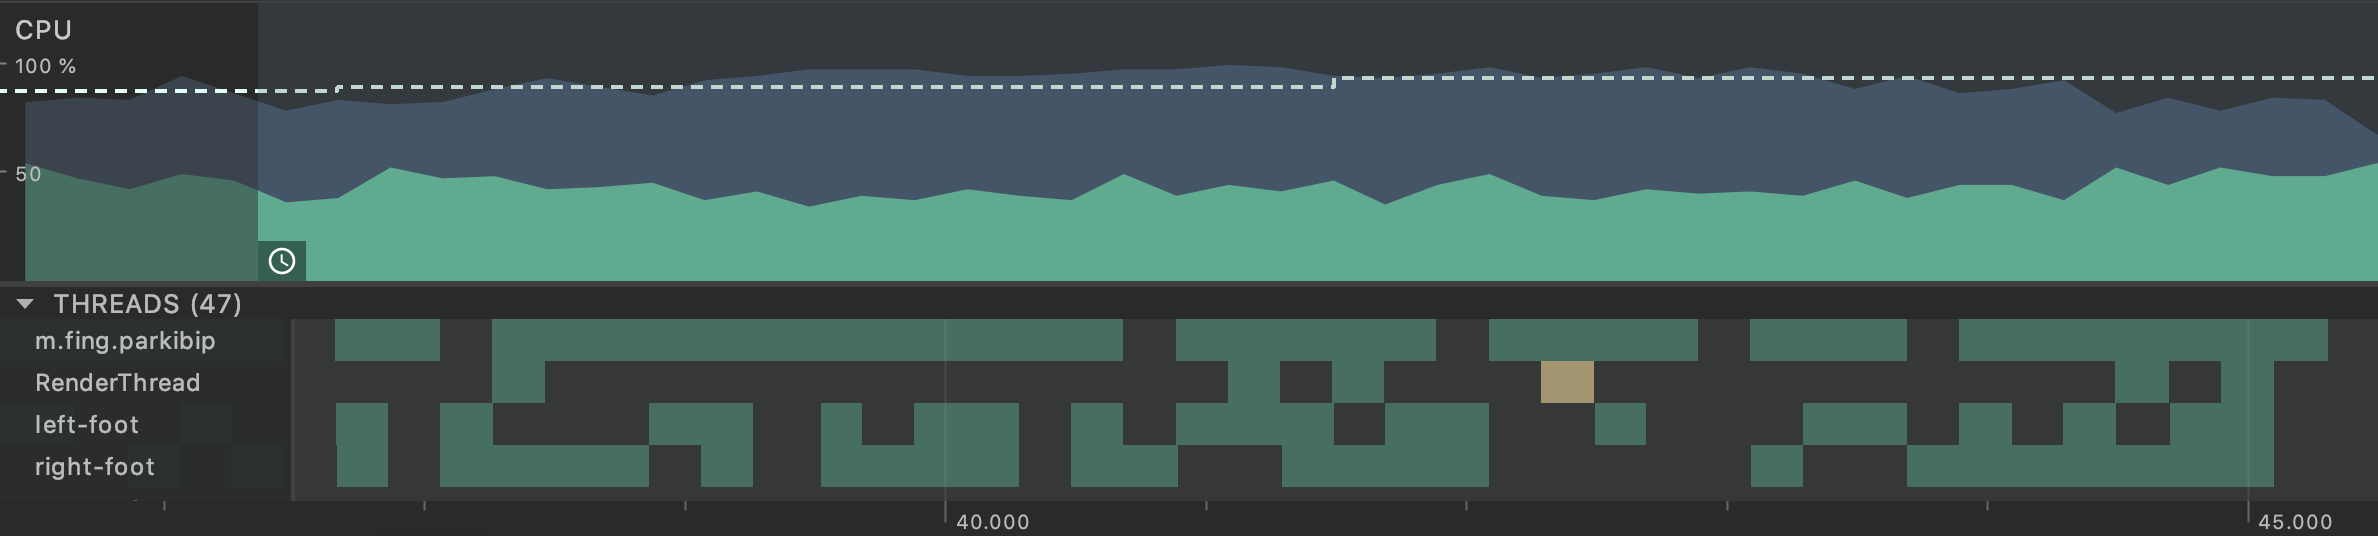
\includegraphics[width=\textwidth]{TESIS/imagenes/chap06/cpu-usage-general.png}
\caption{Porcentaje de utilización de la Unidad Central de Procesamiento (CPU) de PARKIBIP analizando datos de dos dispositivos a 400Hz -en verde-. Pico máximo de 56\% de uso. En la parte inferior se puede ver la utilización de la CPU para los distintos hilos de ejecución. En gris se puede ver el uso de la CPU de otras aplicaciones del sistema. Esta gráfica se obtiene utilizando la herramienta \textit{Profiler} de Android Studio.}
\label{FIG:CPU-usage}
\end{figure}

Como se puede observar en la figura, los hilos ``left-foot'' y ``right-foot'', dedicados al procesamiento de los datos para cada dispositivo, están quitando una carga considerable al hilo principal. Además, estos no están realizando un uso extensivo de la CPU, ya que realizan procesamiento en intervalos cortos y eficientes. 

Adicionalmente, se puede utilizar esta herramienta para investigar el uso que se está realizando de cada hilo, es decir, cuáles son las instrucciones que se están ejecutando en cada hilo y cuáles son aquellas que están demandando más tiempo a este recurso. La figura \ref{FIG:cpu-usage-threads} muestra las instrucciones que están siendo ejecutadas en un instante de tiempo determinado, durante una sesión de terapia activa.

\newpage

\begin{figure}[H]
\hspace{-2.0cm}
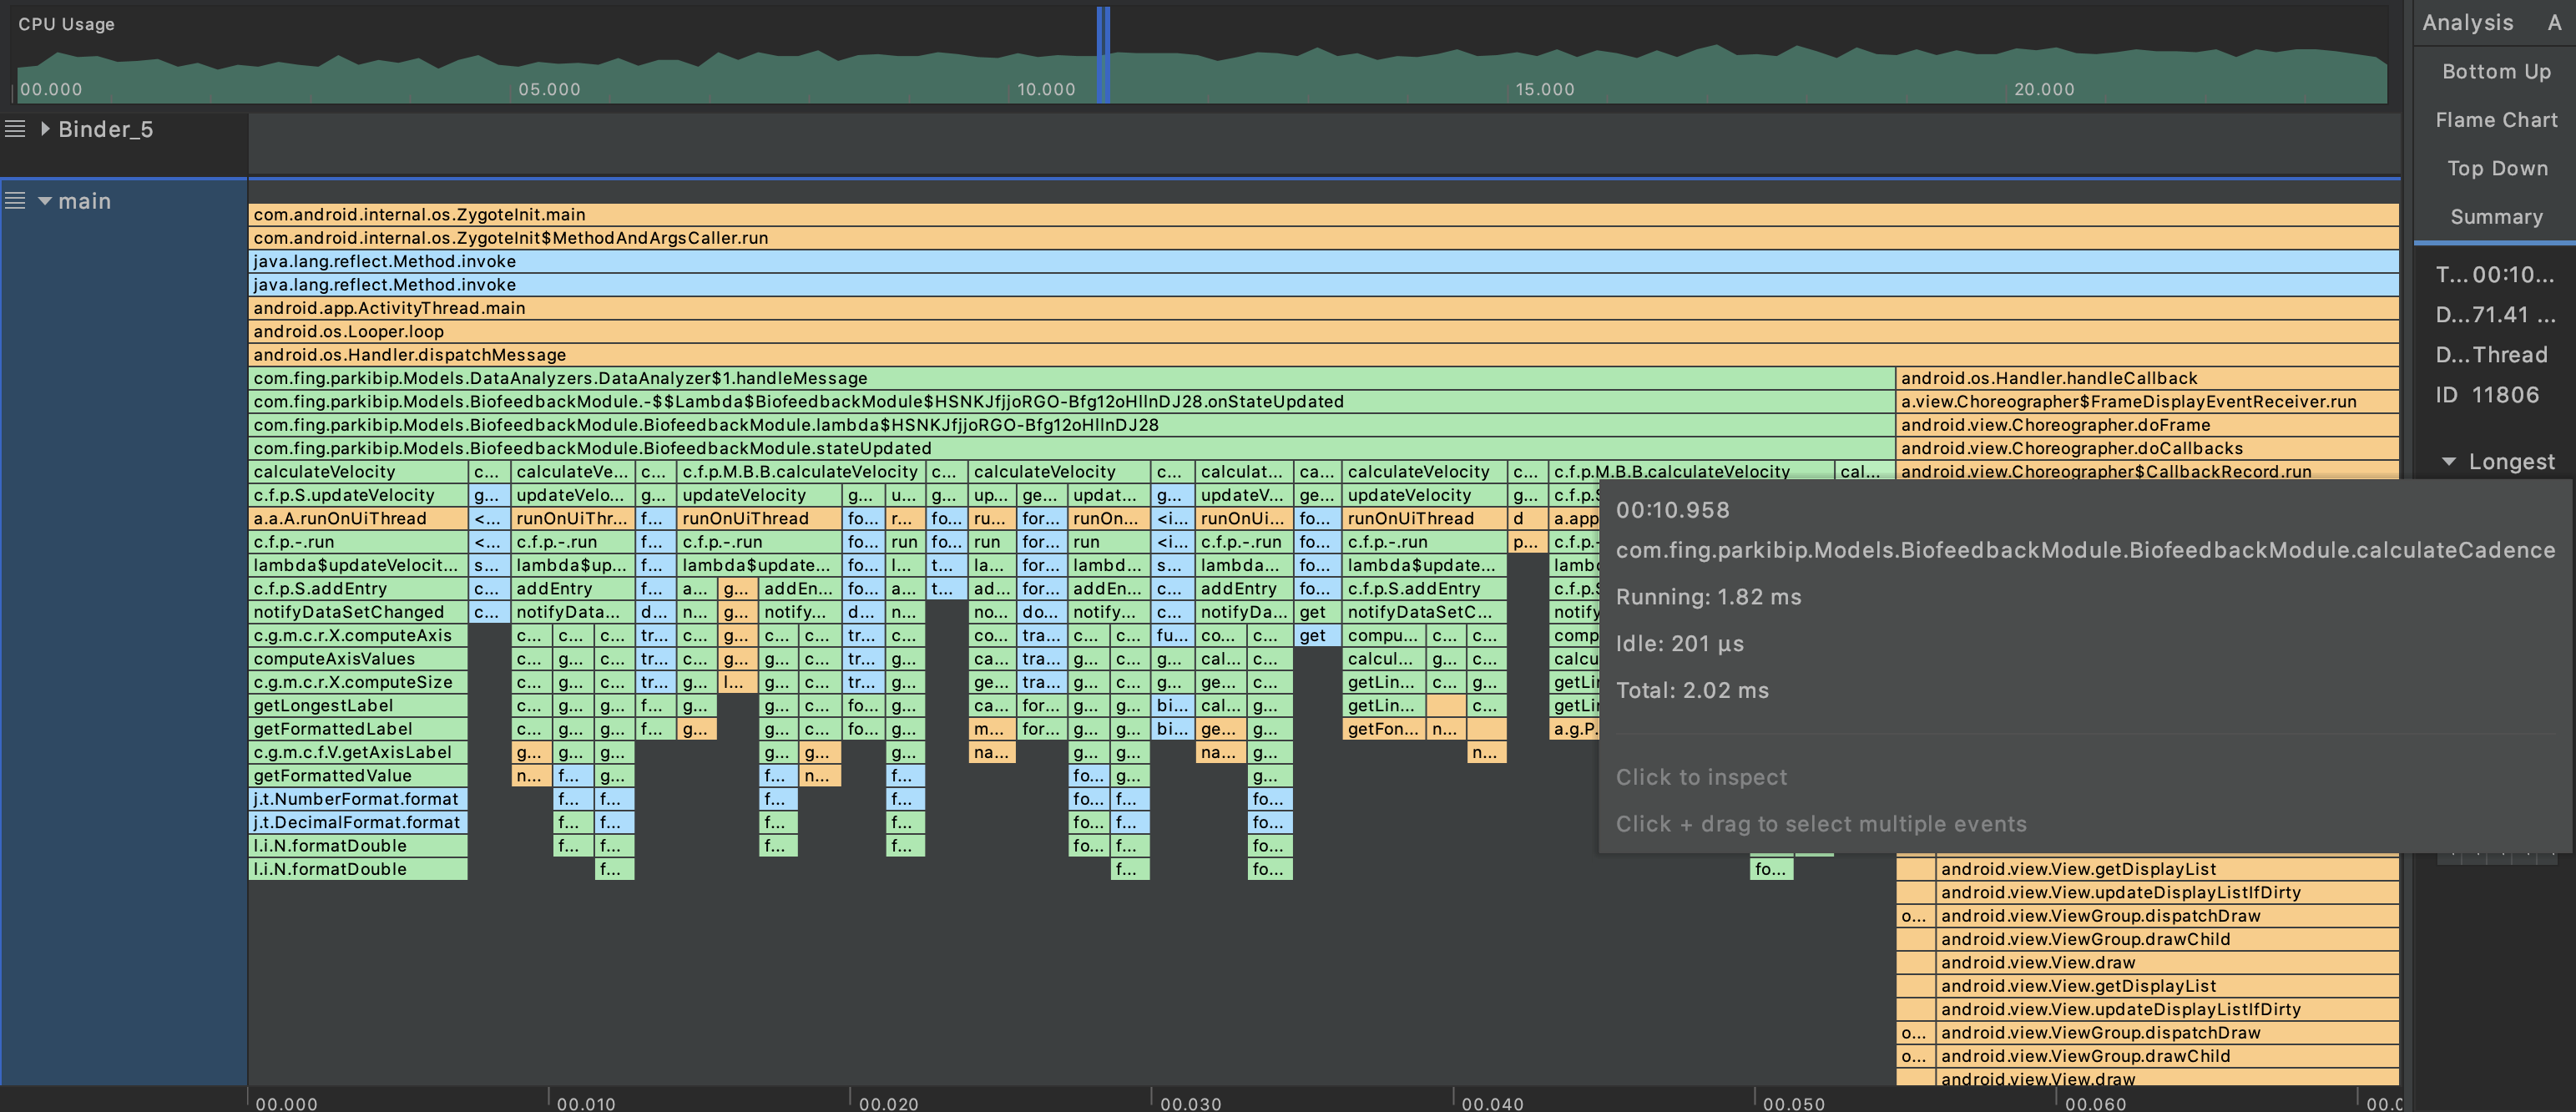
\includegraphics[clip,width=1.3 \columnwidth]{TESIS/imagenes/chap06/cpu-usage-threads.png}
\caption{Ejemplo de instrucciones ejecutadas en un instante de tiempo dado por PARKIBIP en un hilo específico. En este caso estas instrucciones se ejecutan en el hilo principal. Es posible seleccionar una de estas instrucciones para ver más detalles. Esta gráfica se obtiene utilizando la herramienta \textit{Profiler} de Android Studio.} 
\label{FIG:cpu-usage-threads}
\end{figure}

La herramienta permite, esencialmente, indagar en los momentos específicos en los que un hilo está siendo sobrecargado. Así, detectar cuáles son las instrucciones que se están ejecutando y qué tiempo de procesamiento están necesitando para completarse. 

Cabe destacar, que durante el análisis de uso de CPU, se detectó que en el escenario 3 la aplicación respondía de forma lenta a las interacciones del usuario. Esto se debía a que se estaba actualizando la interfaz gráfica de la pantalla de sesión activa de forma instantánea por cada dato recibido, resultando en un uso exhaustivo del hilo principal. Para corregir la problemática, se modificó la implementación para que las actualizaciones ocurran cada $f$ datos, siendo $f$ un número configurable. Si bien los parámetros se calculan elemento a elemento, las actualizaciones en pantalla se realizan cada $f$ elementos. La selección de dicho número se realiza en función de la frecuencia de datos que provee el sensor, de forma que se mantenga una percepción de tiempo real sin saturar el hilo principal.
\newline \newline

\section*{Memoria}

Otro aspecto importante es, el uso de la memoria que realiza la aplicación. Es importante que la aplicación no esté haciendo un mal uso de este recurso, ya que puede derivar en una degradación de la aplicación e incluso de todo el \textit{smartphone}. Para ésto, se monitorean las reservas de memoria (a.k.a. \textit{allocs}) que realiza la aplicación en tiempo real, utilizando también la herramienta \textit{Profiler}. 

Los aspectos fundamentales a evaluar en cuanto al uso de la memoria son: 

\begin{itemize}
    \item Si la memoria que ya no se utiliza está siendo liberada adecuadamente
    \item Si no se está usando memoria de forma innecesaria
\end{itemize}

Para verificar el primer punto, se supervisa la memoria con \textit{Profiler} durante la apertura de una pantalla en la aplicación. Se verifica que, una vez que se cierra dicha pantalla, la memoria ocupada al abrirla vuelve a liberarse. Esto se realiza para cada una de las pantallas o \textit{Activities}. Luego, se estudió detalladamente en qué se está utilizando la memoria en cada momento, con el objetivo de evitar el uso innecesario de la misma. Se detectó que las listas de mediciones mantenidas en memoria estaban ocupando grandes cantidades de almacenamiento, por lo que se disminuyeron los intervalos de tiempo para realizar el guardado en la base de datos y de esta forma evitar mantener tantas mediciones en memoria. La figura Fig. \ref{FIG:memory-usage} muestra la gráfica de uso de memoria durante el procesamiento en tiempo real. El pico máximo de memoria utilizada fue de 62MB.

\begin{figure}[H]
\centering
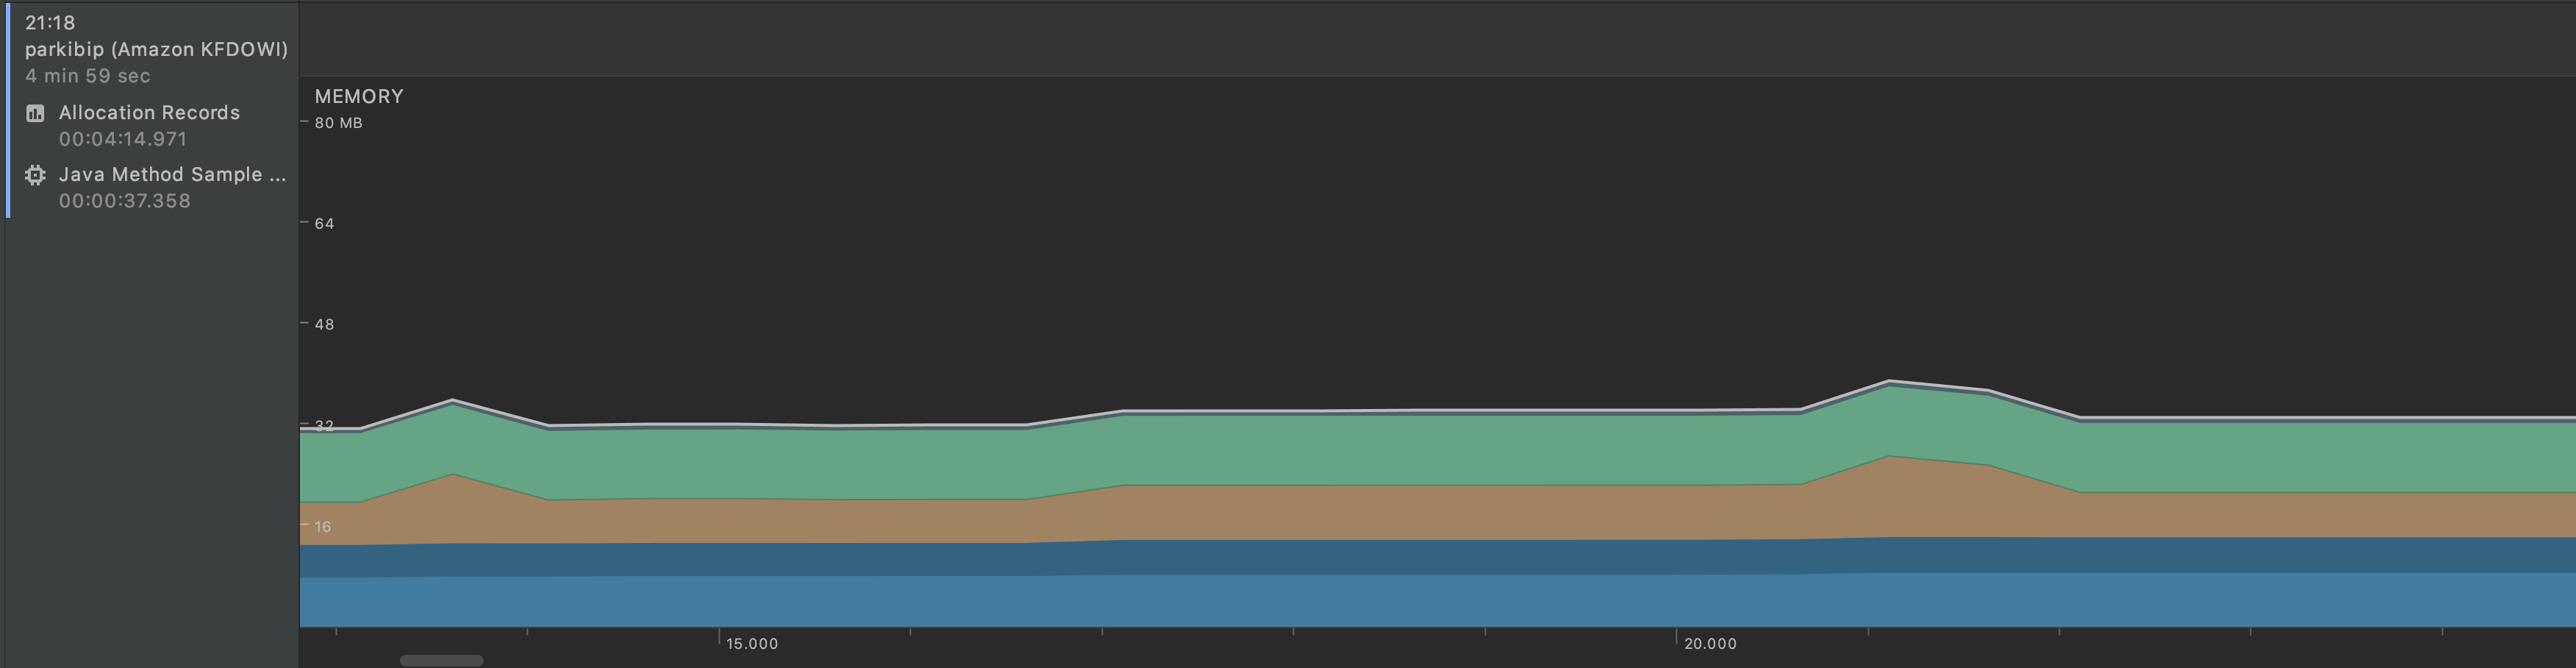
\includegraphics[width=\textwidth]{TESIS/imagenes/chap06/memory-usage.png}
\caption{Ejemplo de uso de memoria utilizada por PARKIBIP durante el procesamiento de los datos. Esta gráfica se obtiene utilizando la herramienta \textit{Profiler} de Android Studio.}
\label{FIG:memory-usage}
\end{figure}

\section*{Uso de Batería}

Analizando el uso de la batería no se detectó ningún tipo de anomalía. El uso de la batería, es categorizado por \textit{Profiler} como Liviano, Medio o Pesado. Para PARKIBIP, en el flujo con mayor procesamiento -sesión activa en curso-, el uso de la batería fue de nivel Medio, y en el resto de los flujos fue Liviano. El diagrama de la figura Fig. \ref{FIG:battery-usage} expone el uso de la batería durante una sesión activa.

\begin{figure}[H]
\hspace{-2.0cm}
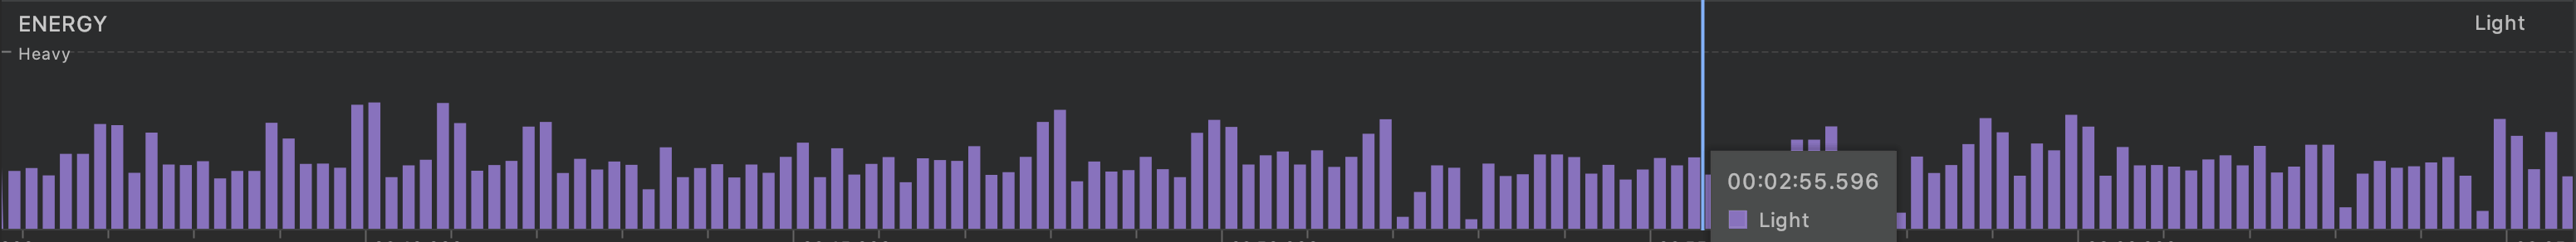
\includegraphics[clip,width=1.3 \columnwidth]{TESIS/imagenes/chap06/battery-usage.png}
\caption{Porcentaje de uso de batería en tiempo real durante una sesión activa de PARKIBIP. En promedio el uso es de la batería es de nivel Medio en esta etapa.}
\label{FIG:battery-usage}
\end{figure}

\section{Asociación Uruguaya de Parkinson}

En virtud de las necesidades de recolección de datos espacio-temporales -relativa a los sujetos con la EP para su posterior análisis-, realizar un estudio observacional de los participantes en diferentes sesiones -para un análisis cualitativo- y evaluar el uso del sistema en tiempo real; se contactó a la \gls{aup} con el fin de cubrir dichos requerimientos.

La AUP es una organización sin fines de lucro, presidida por la Sra. Ana Ma. Martinez, orientada a (i) contribuir en la investigación y la elaboración de material teórico y práctico sobre calidad de vida e intervención en grupos terapéuticos para personas con EP y sus familiares, (ii) contribuir al desarrollo de calidad de vida. En la misma, se realizan diversas actividades grupales con los sujetos afectados en reuniones semanales -presenciales y no presenciales-, tales como clases de yoga, canto, estiramiento, trabajos cognitivos y de memoria, terapias con voluntarios especializados (i.e. fisioterapeutas), etc.

Con la autorización adecuada de la presidente de la AUP y la posterior redacción de un consentimiento informado -anexo del presente informe, \nameref{anexo:Consentimiento}-, procedimiento mediante el cual se garantiza que el sujeto ha expresado voluntariamente su intención de participar en la investigación y comprendido la información que se le ha dado acerca de los objetivos y los beneficios de la misma; se procedió a establecer sesiones guiadas de análisis y recopilación de datos. 

\section{Población y protocolo experimental}\label{aup:sesiones}

Quince voluntarios reclutados de la AUP con la enfermedad de Parkinson participaron en este estudio demostrando absoluto interés e ilusión en la investigación. El procedimiento  para la extracción de las características de la marcha fue realizado bajo el acompañamiento de un Lic. en Fisioterapia, luego de que el protocolo y el consentimiento fueran aprobados.

Durante el mes de Diciembre del 2019, un total de 8 parkinsonianos masculinos y 7 femeninos emplearon el sistema PARKIBIP -15 participantes-, con una edad promedio de 74.5 años (mínima: 57, máxima: 85), marcha independiente y de distintas zonas barriales de Montevideo-Uruguay. Todos los sujetos realizaron una caminata lineal en un suelo plano -sin alteraciones- y con marcha normal hacia adelante. Los datos del acelerómetro, el giroscopio y el magnetómetro de los dispositivos IMU conectados, ubicados en los talones de los pies del participante, fueron registrados. La distancia recorrida por participante fue de 10 metros, medida a través de marcas en el piso, totalizando un total de 150 metros. La figura Fig. \ref{fig:real-session-aup} expone una fotografía tomada durante una de las sesiones desarrolladas con voluntarios de AUP, además se adjunta una grabación de una sesión PARKIBIP \footnote{Las grabaciones circulares se encuentran disponibles en el sitio  \href{https://drive.google.com/drive/folders/1qmg-Nex1i13uaCr66KOUZ3LE5vgFuK2W?usp=sharing}{PARKIBIP-grabaciones-circulares}
}. 

\begin{figure}[h!]
\centering
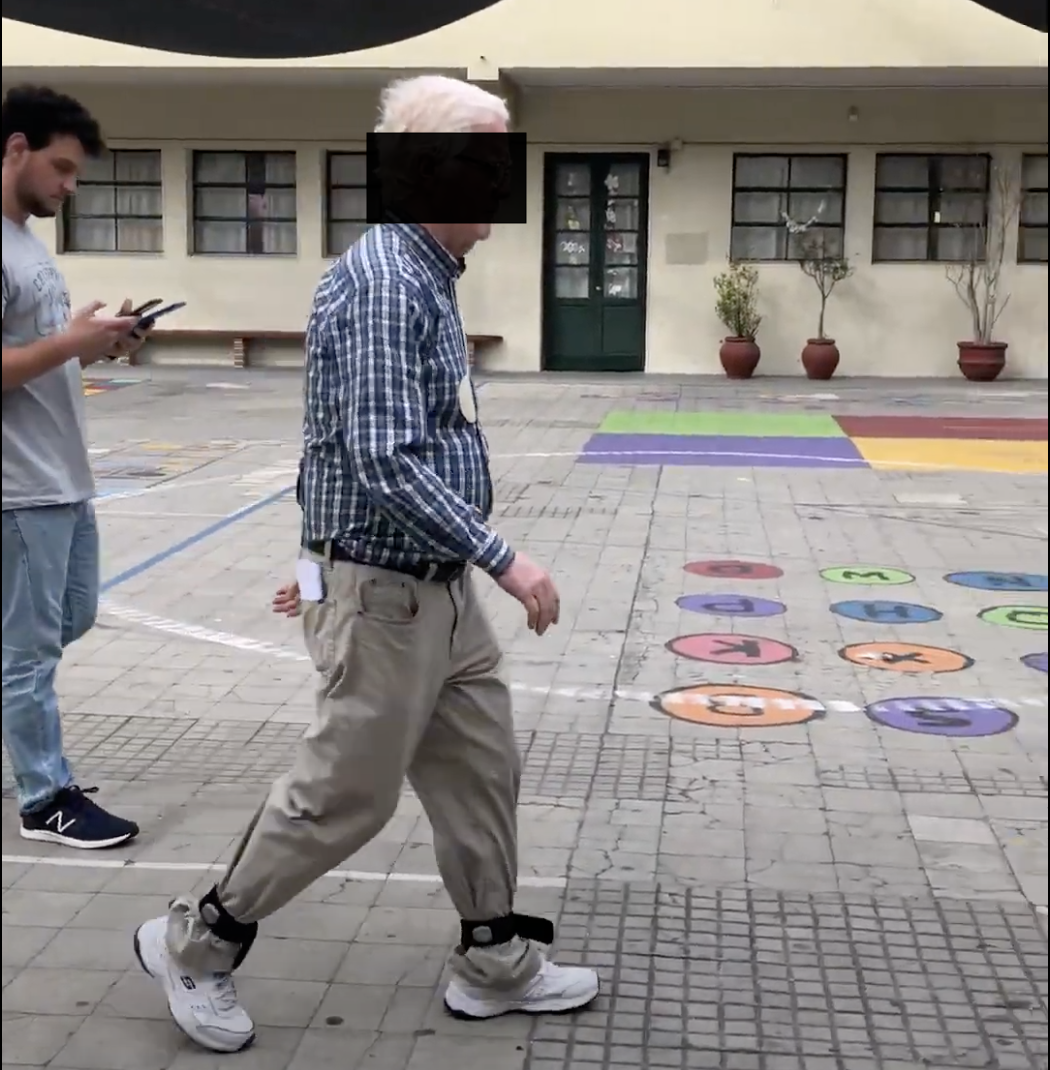
\includegraphics[clip,width=0.6 \columnwidth]{TESIS/imagenes/chap06/aup-session-image.png}
\caption{Foto tomada durante una de las sesiones desarrolladas con voluntarios de AUP. Diciembre, 2019.}
\label{fig:real-session-aup}
\end{figure}

Asimismo, para cada parkinsoniano voluntario se efectuó un cuestionario, con el objetivo de registrar información relativa a la patología (i.e. tipo de parkinson), información personal (i.e. nombre completo,  teléfono de contacto, continuidad en la participación), si asistían o asistieron al programa PRENPAR -Programa de Educación y Rehabilitación en la Enfermedad de Parkinson para pacientes, familiares y cuidadores-, si frecuentaban el centro Hospital de Clínicas, entre otras.

\newpage

\section{Toma de datos obtenidos en lazo abierto (AUP)}

Con el fin de presentar los resultados adquiridos, el análisis se organiza según el orden cronológico de ciertas actividades:
\begin{enumerate}
    \item En el mes de Diciembre de 2019, se evalúa la recolección de datos inerciales de enfermos de Parkinson, con el sistema PARKIBIP (i.e. integrantes  de la AUP). Dichos datos fueron esenciales para trabajar durante el proyecto.
    \item El proyecto PARKIBIP fue presentado y evaluado en funcionamiento por voluntarios en el congreso y pre-congreso latinoamericano de Ingeniería Biomédica SABI 2020 (por sus siglas, Sociedad Argentina de Bioingeniería), paper científico mediante -marzo del 2020-.
    \item Luego, se propone evaluar el comportamiento de PARKIBIP con un sistema de referencia y obtener métricas comparativas.
    \item Para finalizar, se analiza la marcha de sujetos sin afecciones, y se realizan reflexiones generales del uso de PARKIBIP.
\end{enumerate}

Las pruebas iniciales consistieron en recuperar, consolidar y almacenar en una base de datos local al dispositivo, las mediciones inerciales de parkinsonianos con PARKIBIP. Los propósitos de dichas pruebas fueron: (i) evaluar el funcionamiento de los sensores IMU en la aplicación, (ii) verificar el almacenamiento de datos inerciales asíncronos, (iii) validar el rendimiento de PARKIBIP (e.g. cuánto soporta la misma, en términos de fallas), (iv) por ultimo y no menos importante, aproximarse y comprender la enfermedad. Tal como se menciona en \nameref{aup:sesiones}, para llevar a cabo los objetivos, se realizaron diversas sesiones de caminatas con integrantes de la asociación.

\noindent Primero y principal, la operación de PARKIBIP fue exitosa y todos los objetivos fueron cumplidos satisfactoriamente. El sistema, soporto adecuadamente 15 sesiones con sujetos diferentes, recopilando y procesando un total de 29.705 muestras de las extremidades inferiores -pies-. No se encontraron anomalías en las pruebas. 

A continuación, se analizan algunas consecuencias logradas y se ejemplifica para la marcha de un sujeto particular. La persona se encuentra inicialmente en reposo, camina 10 metros y vuelve al reposo.

La figura Fig. \ref{fig:acceleration-components} muestra el comportamiento de la aceleración del dispositivo en sus tres componentes, $a_X$ -aceleración en x-, $a_Y$, -aceleración en y- $a_Z$ -aceleración en z-, en las unidades gravitacionales (g) en el sistema internacional. Primero, el acelerómetro mide tanto la aceleración del usuario como la gravitatoria, la componente $a_Y$ dada por la línea negra resalta la afectación de las fuerzas gravitatorias  -iniciando aproximadamente en $-1g$- y así, ese eje se encuentra proyectado en $-1g$. Segundo, se puede apreciar claramente un patrón de comportamiento repetitivo para la marcha, inicia con el pie estacionario -todas las aceleraciones aproximadamente en 0-, presenta un pequeño pico de aceleración vinculado a la fase \textit{midswing} del ciclo, luego, otro pico mas acentuado desde el \textit{midswing} al \textit{HS} (i.e. recordando, heel strike), finalizando con el pie estacionario nuevamente -stance-. Asimismo, es claro un bloqueo de la marcha (i.e. FoG) entre las medidas 610-730, luego dos pasos, y nuevamente un bloqueo para las muestras 840-960.

\begin{figure}[h!]
\hspace*{-2.9cm}%
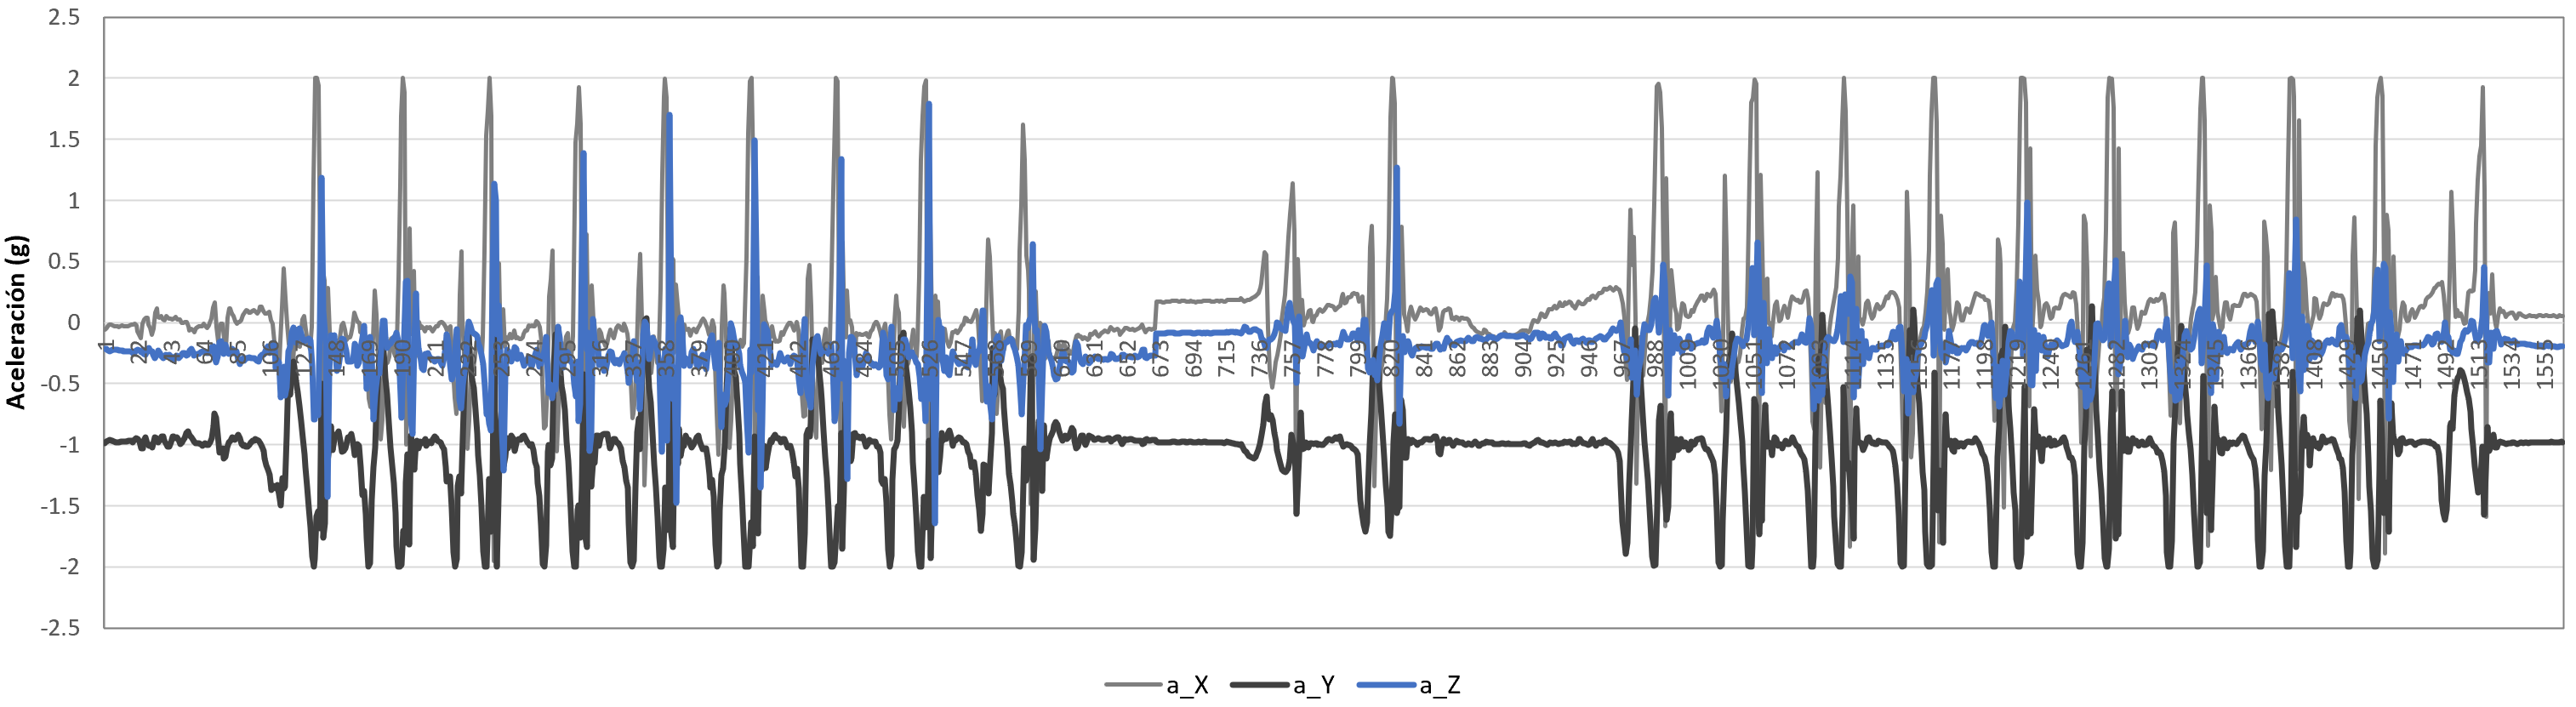
\includegraphics[clip,width=1.4 \columnwidth]{TESIS/imagenes/chap06/acceleration-components.PNG}
\caption{Aceleración tridimensional de un parkinsoniano en el marco del sensor. Representadas por las componentes $a_X$ -aceleración en x-, $a_Y$, -aceleración en y- $a_Z$ -aceleración en z-; en las unidades gravitacionales en el sistema internacional.}
\label{fig:acceleration-components}
\end{figure}

\newpage

Por otro lado, la figura Fig. \ref{fig:acceleration} muestra el resultado de dos métodos que computan la aceleración lineal del usuario en un instante dado, fruto de la rotación de las componentes de la aceleración desde el marco Sensor al marco Tierra -obtenidas del IMU, ver \ref{fig:acceleration-components}-, la extracción de las fuerzas gravitatorias, y luego el cálculo de la norma del vector aceleración resultante. El primer procedimiento, línea azul de la gráfica, emplea el filtro de Orientación -útil en la rotación- únicamente con los datos del acelerómetro y del giroscopio. El segundo método, dado por la línea gris de la gráfica, integra además, el sensor magnetómetro. Así, se observan las consecuencias:

\begin{itemize}
    \item Al integrar datos de fuerzas magnéticas, la calibración de la orientación del sensor, previa al procesamiento, es instantánea. Evaluando la gráfica, se observa que el método que no emplea magnetómetro tarda aproximadamente 100 observaciones en estabilizarse a cero. Se puede concluir que, integrar datos de fuerzas magnéticas resulta en un calculo mas eficiente de orientación.
    \item Asimismo, la gráfica expone un patrón de comportamiento repetitivo, en donde el pico más alto representa un paso del sujeto y los momentos cercanos a cero, momentos estacionarios.
\end{itemize}

\begin{figure}[h!]
\hspace*{-2.9cm}%
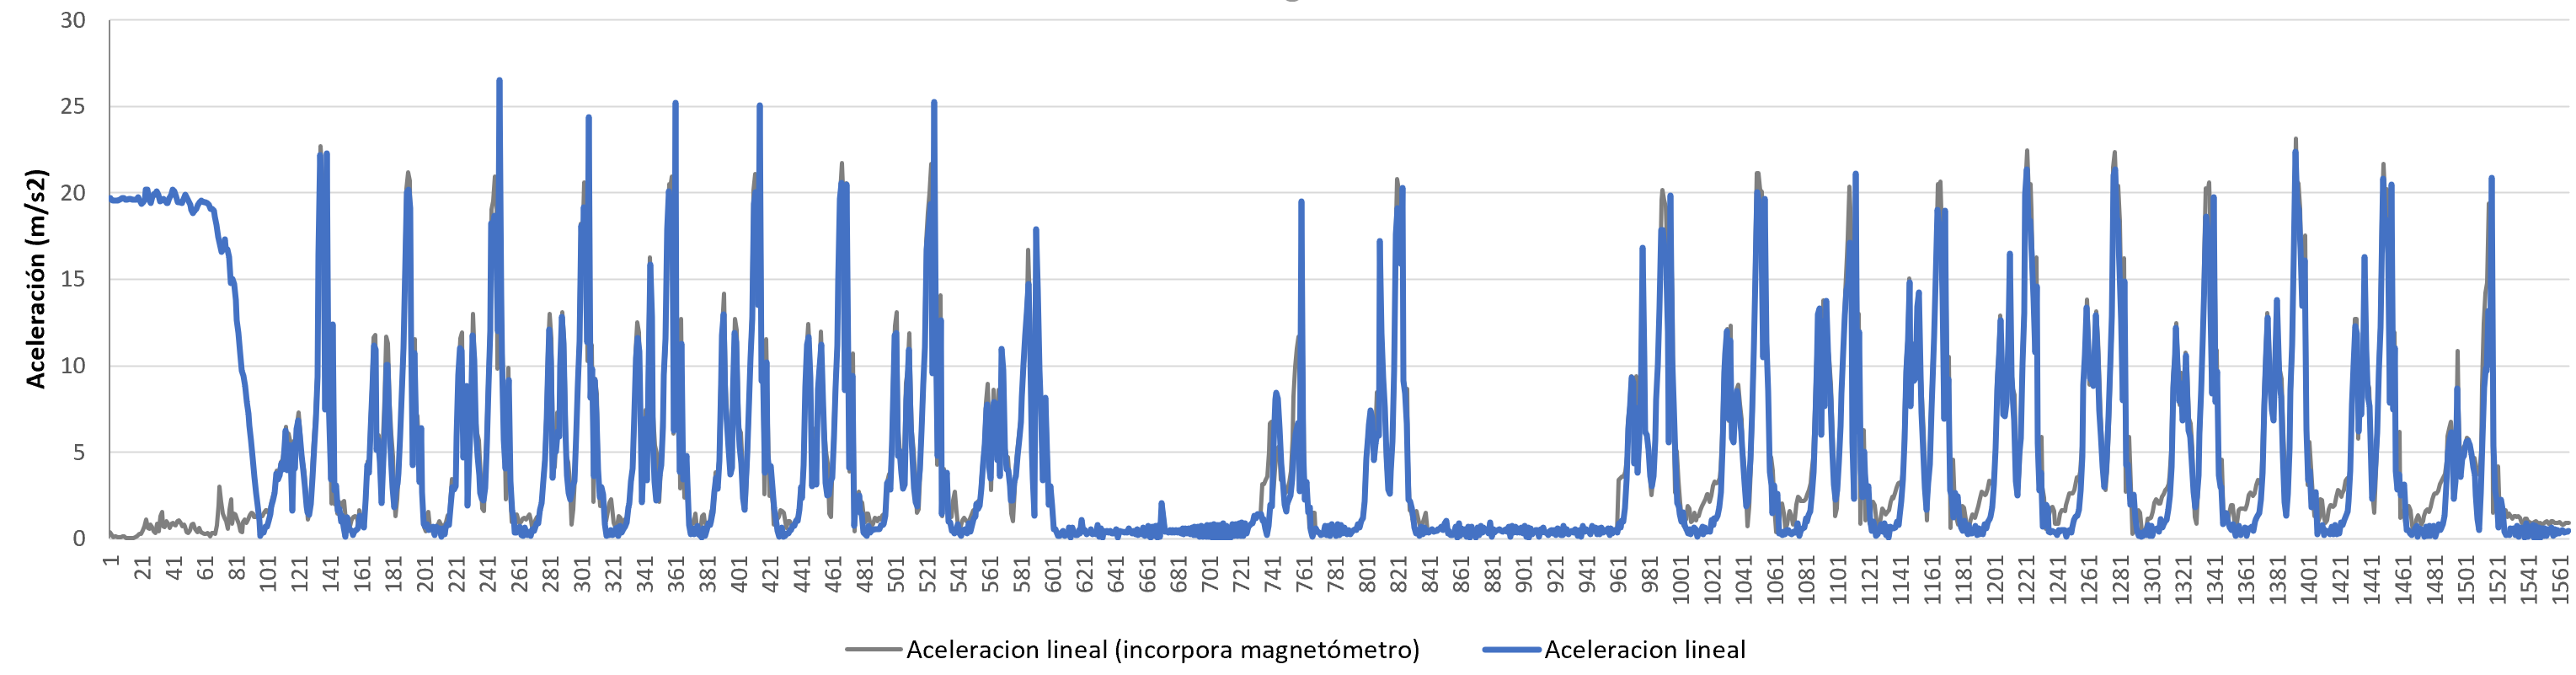
\includegraphics[clip,width=1.4 \columnwidth]{TESIS/imagenes/chap06/linnear-acceleration.PNG}
\caption{Aceleración lineal de un parkinsoniano en el marco de referencia Tierra. Representada en las unidad en el sistema internacional $m/s$.}
\label{fig:acceleration}
\end{figure}

A su vez, fueron evaluados dos aspectos fundamentales de la marcha del sujeto. Por un lado el ciclo conformado por sus fases Stance/Swing, por otro la velocidad instantánea adquirida en $m/s$. La figura Fig. \ref{fig:zvd-velocity}, superpone ambos resultados en dicha gráfica. Primero, la línea superior bordo indica los estados estacionarios o de velocidad cero -detectados con el método MV de ZVD-, mientras que la línea inferior del mismo color, la transición al movimiento. Así, se detectan las fases HS, como la transición de 0 a 0.5 -en la gráfica-, y la fase TO, como la transición inversa. Segundo, dada por la linea azul, se expone la velocidad del usuario, en la unidad del sistema internacional $m/s$. Se aprecia que ambos resultados son consistentes, ya que cuando la velocidad es cero, el pie del usuario se encuentra estacionario.
\noindent De manera complementaria, se reconocen ciertos falsos positivos, previos al valor 581. Esto, se debe a la fecha temprana de las pruebas, y que no fueron recopilados datos del magnetómetro en esta etapa -útil para la eficiencia del filtro de orientación-.

\begin{figure}[h!]
\hspace*{-2.9cm}%
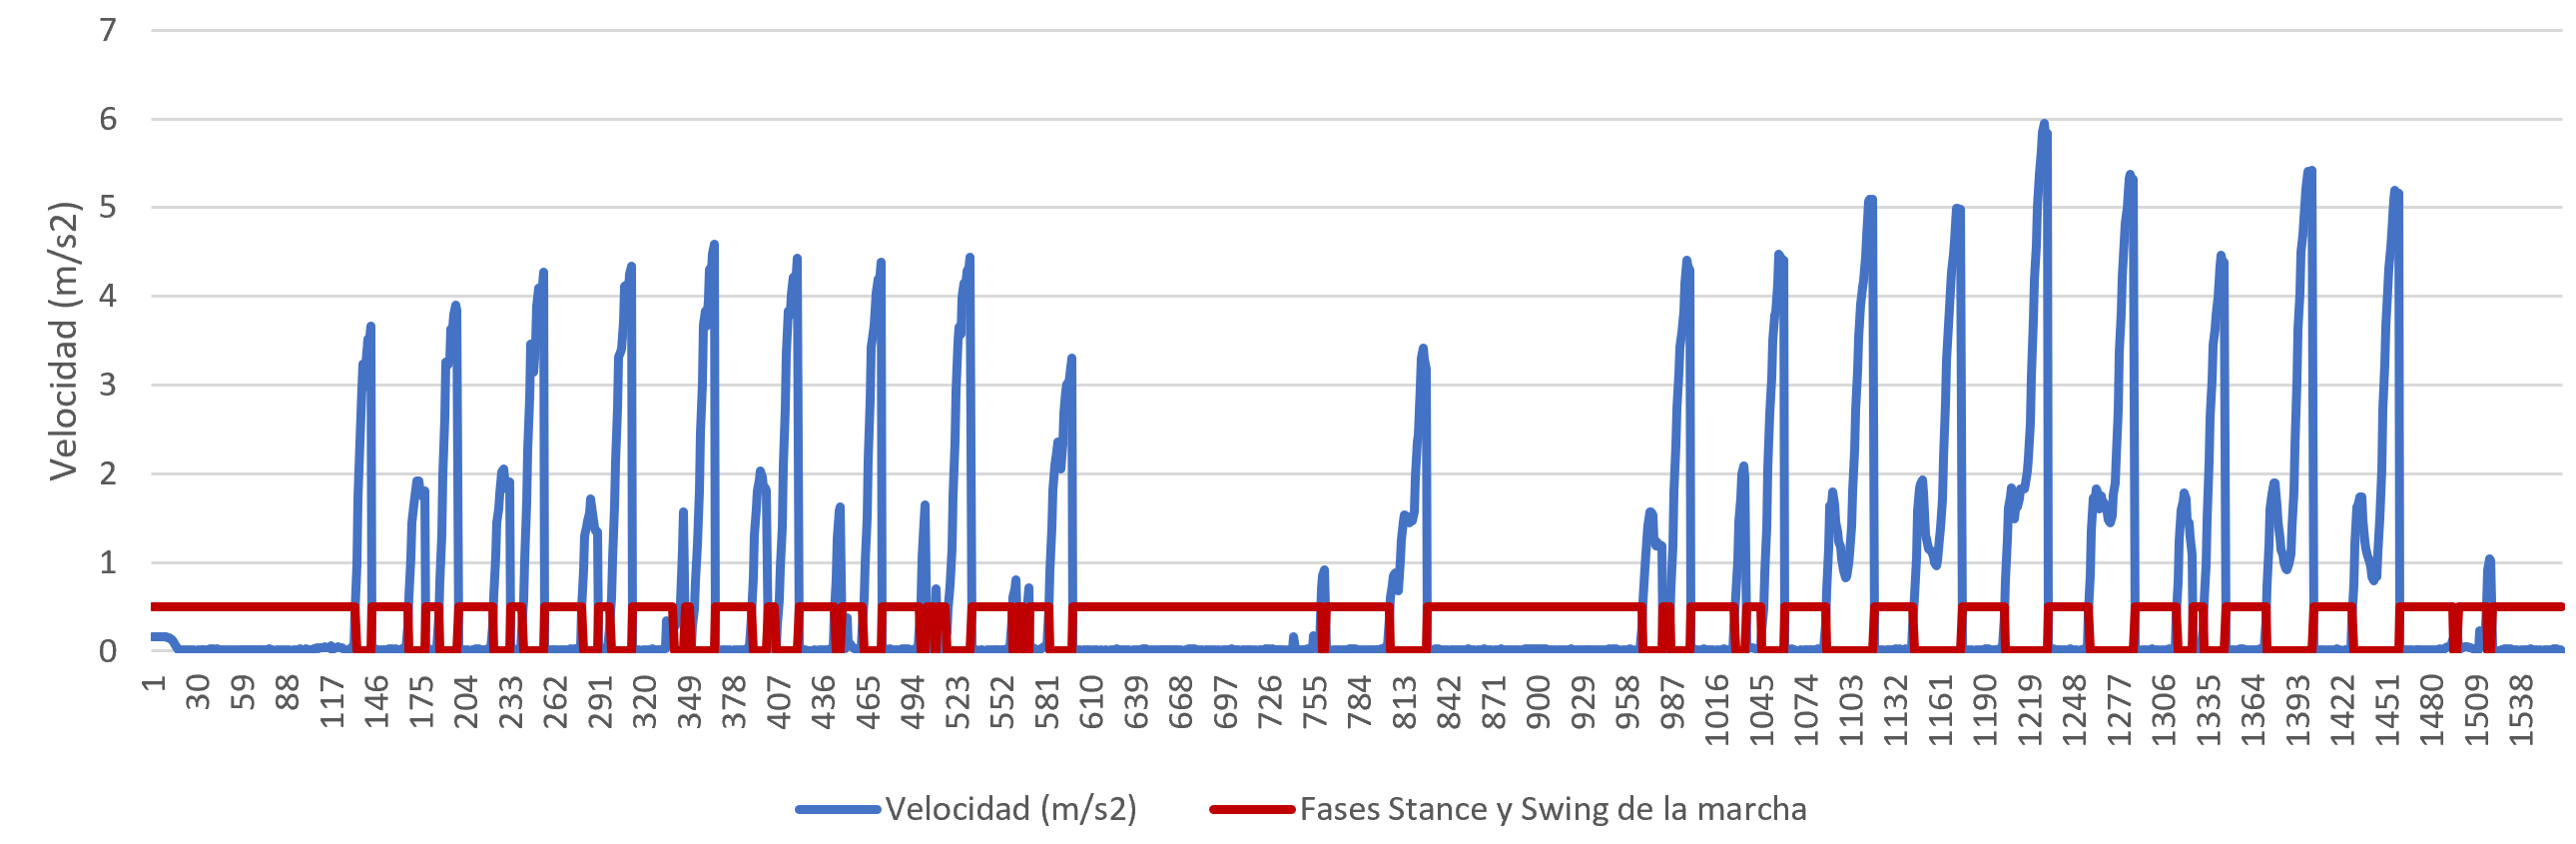
\includegraphics[clip,width=1.4 \columnwidth]{TESIS/imagenes/chap06/velocity-zvd.PNG}
\caption{Velocidad del usuario en $m/s^2$ y detecciones de velocidad cero. La linea bordó indica las transiciones de desde el estado estacionario -nivel superior- al estado en movimiento -nivel inferior-.}
\label{fig:zvd-velocity}
\end{figure}

Finalmente, se obtuvo una velocidad media de 0.73 $m/s$ para dicho sujeto.

Hay que mencionar además que, se lograron mejores resultados en la rotación del vector tridimensional en el marco de referencia del Sensor, hacia el marco de coordenada inercial Tierra, con el factor de convergencia $\beta$ igual a 5. En PARKIBIP y con el IMU Metawear, factores de $\beta$ bajos conllevaban a errores incrementales en el cómputo del \textit{quaternion}. Este error, luego impactaba negativamente en los parámetros espacio-temporales.

\section{Pruebas de PARKIBIP con estimulación}

Seguido a las pruebas con la AUP, PARKIBIP fue aceptado e invitado a exponer como orador en el congreso SABI 2020, mediante la elaboración de un \textbf{paper de investigación}. El mismo, se puede hallar en el apéndice \nameref{chap:sabi2020}. Durante el transcurso del congreso, PARKIBIP fue evaluado en operativo mediante voluntarios vinculados a la ingeniería biomédica. Tres participantes emplearon PARKIBIP por medio de marchas lineales en una superficie plana y un estímulo de vibración configurado en cada pisada (un ingeniero biomédico de origen peruano, un médico argentino y un profesor de educación física uruguayo). El sistema actuó correctamente, estimulando al usuario con cada pisada. A su vez, el feedback recibido por los participantes fue positivo y alentador.

\section{Evaluación de PARKIBIP con sistema de referencia}

Conforme a evaluar el sistema frente a algún sistema de referencia, fue propuesto el laboratorio de marcha y su sistema VICON 3D del Hospital de Clínicas. Sin embargo, se presentaron ciertas limitantes del contexto: (i) pandemia de Covid-19 de por medio, (ii) complejidad en el acceso al laboratorio especializado, (iii) dificultad en la obtención de pacientes habilitados, (iv) en general, los pacientes son mayores, y pertenecen a la población de riesgo. Así, PARKIBIP fue evaluado usando datos inerciales \textit{Open Source} en el lenguaje de desarrollo Matlab, propiedad de \textit{OpenShoe} \cite{openshoe}.

Se procesaron 12.239 observaciones, tomadas del IMU  MicroStrain 3DX-GX2 con una frecuencia de 250Hz. El IMU fue montado en la suela del zapato del lado derecho del usuario, y el mismo camino simulando una trayectoria de circuito cerrado. Se tienen como valores esperados, la posición inicial igual a la final, la velocidad media de 1.94 m/s.

Se efectuaron las siguientes comparaciones con datos de \textit{OpenShoe}:
\begin{itemize}
    \item Comportamiento entre los métodos de ZVD PARKIBIP (i.e. MV versus GLRT)
    \item Velocidad media PARKIBIP versus velocidad media Openshoe. Cálculo del error cuadrático medio (en inglés, root-mean-square deviation, RMSD)
    \item Trayectoria PARKIBIP versus trayectoria Openshoe
\end{itemize}

La prueba inicial consintió en correr los algoritmos de detección de velocidad cero ZVD-, a través de los dos métodos implementados -MV y GLRT- con los datos ya mencionados. Las figuras Fig. \ref{fig:openshoe-mv} y \ref{fig:openshoe-glrt}, muestran la aceleración lineal del usuario en la unidad gravitacional junto a las detecciones de cero velocidad para ambos métodos. Como se puede observar la primer figura empleando el método MV -Fig. \ref{fig:openshoe-mv}-, presenta un mayor número de detección o transiciones entre estados, que explican varios falsos positivos. Sin embargo, la segunda figura empleando el método GLRT -\ref{fig:openshoe-glrt}- fue mucho mas precisa con las detecciones. \textbf{Como resultado, se puede decir que GLRT es mas preciso que MV, ya que contempla las variaciones en la velocidad angular}.

\begin{figure}[h!]
\hspace*{-2.9cm}%
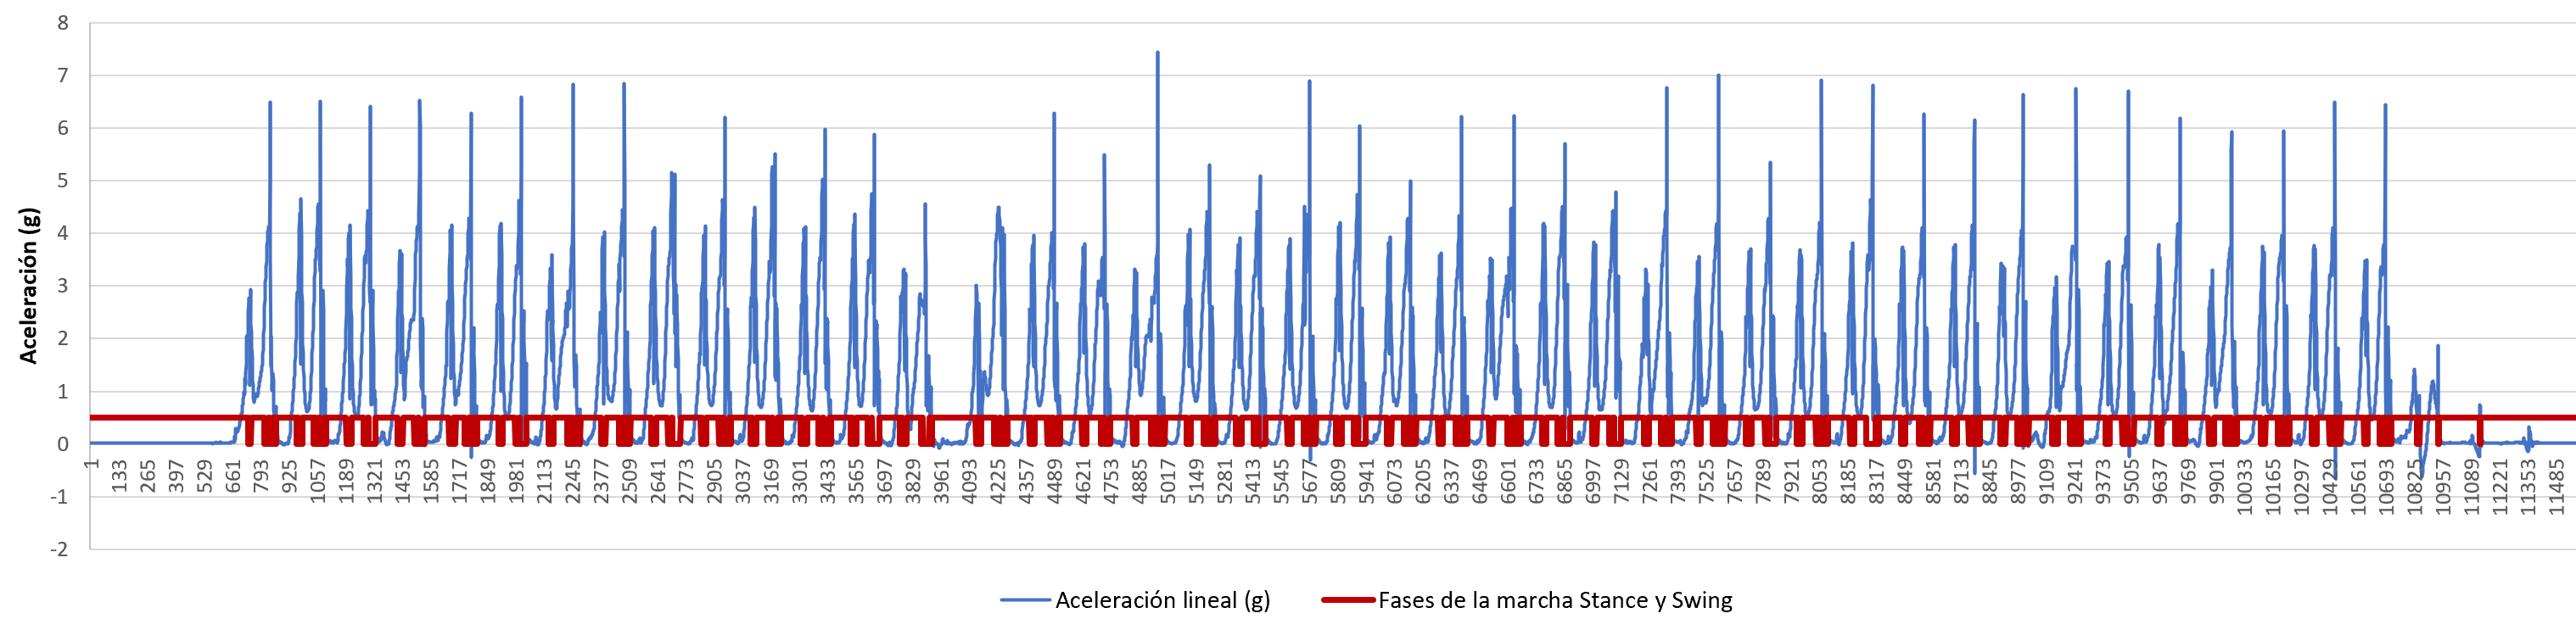
\includegraphics[clip,width=1.4 \columnwidth]{TESIS/imagenes/chap06/acceleration-zvd-openshoe-mv.PNG}
\caption{Aceleración lineal del usuario en $m/s^2$ y detecciones de velocidad cero con el método MV. La linea bordo indica las transiciones de desde el estado estacionario -nivel superior- al estado en movimiento -nivel inferior-.}
\label{fig:openshoe-mv}
\end{figure}

\begin{figure}[h!]
\hspace*{-2.9cm}%
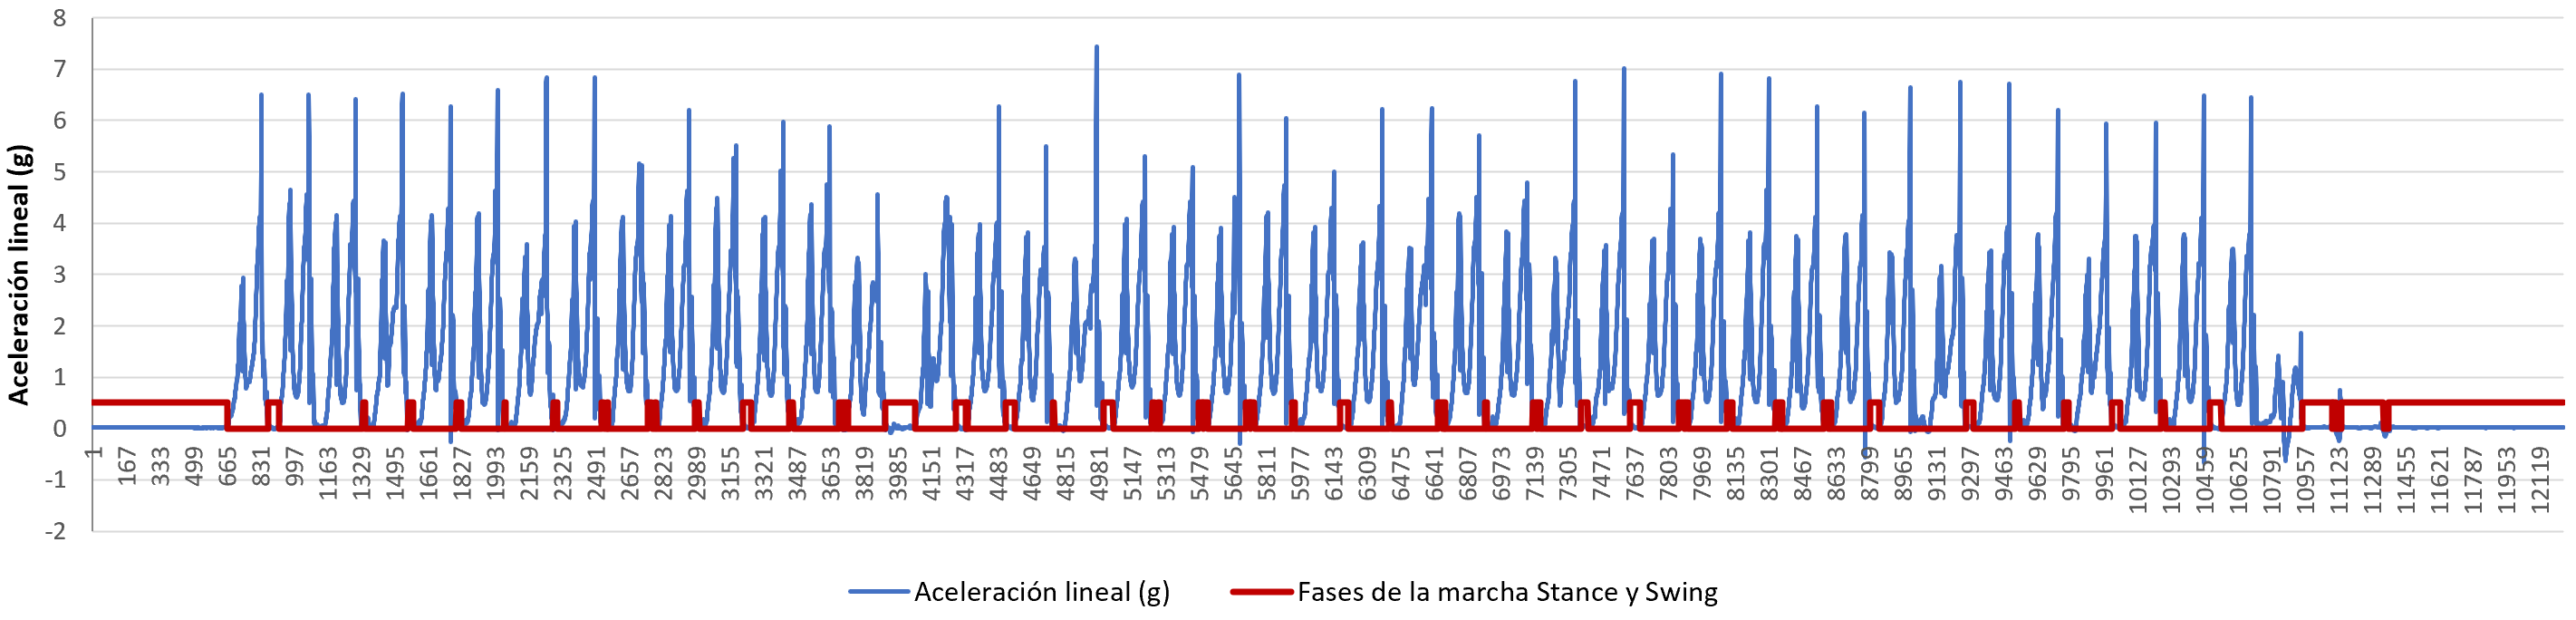
\includegraphics[clip,width=1.4 \columnwidth]{TESIS/imagenes/chap06/acceleration-zvd-openshoe-glrt.PNG}
\caption{Aceleración lineal del usuario en $m/s^2$ y detecciones de velocidad cero con el método GLRT. La linea bordo indica las transiciones de desde el estado estacionario -nivel superior- al estado en movimiento -nivel inferior-.}
\label{fig:openshoe-glrt}
\end{figure}

Además, fueron comparados los parámetros espacio-temporales velocidad media y trayectoria frente a los valores esperados por Openshoe. La imagen Fig. \ref{fig:openshoe-velocity}, exhibe la velocidad del usuario resultado del procesamiento del filtro de Kalman PARKIBIP, en $m/s$. El valor esperado, según la marcha del usuario, es de 1.94 $m/s$. Así, \textbf{la velocidad media lograda por PARKIBIP fue de 1.81$m/s$, indicando una diferencia de 0.13 $m/s$}.  En cambio Openshoe alcanzo un valor de 1.75$m/s$. Como consecuencia del análisis, \textbf{el error cuadrático medio (RSME) entre las velocidades instantáneas de PARKIBIP y Openshoe fue de 0.0214}.

\begin{figure}[h!]
\hspace*{-2.9cm}%
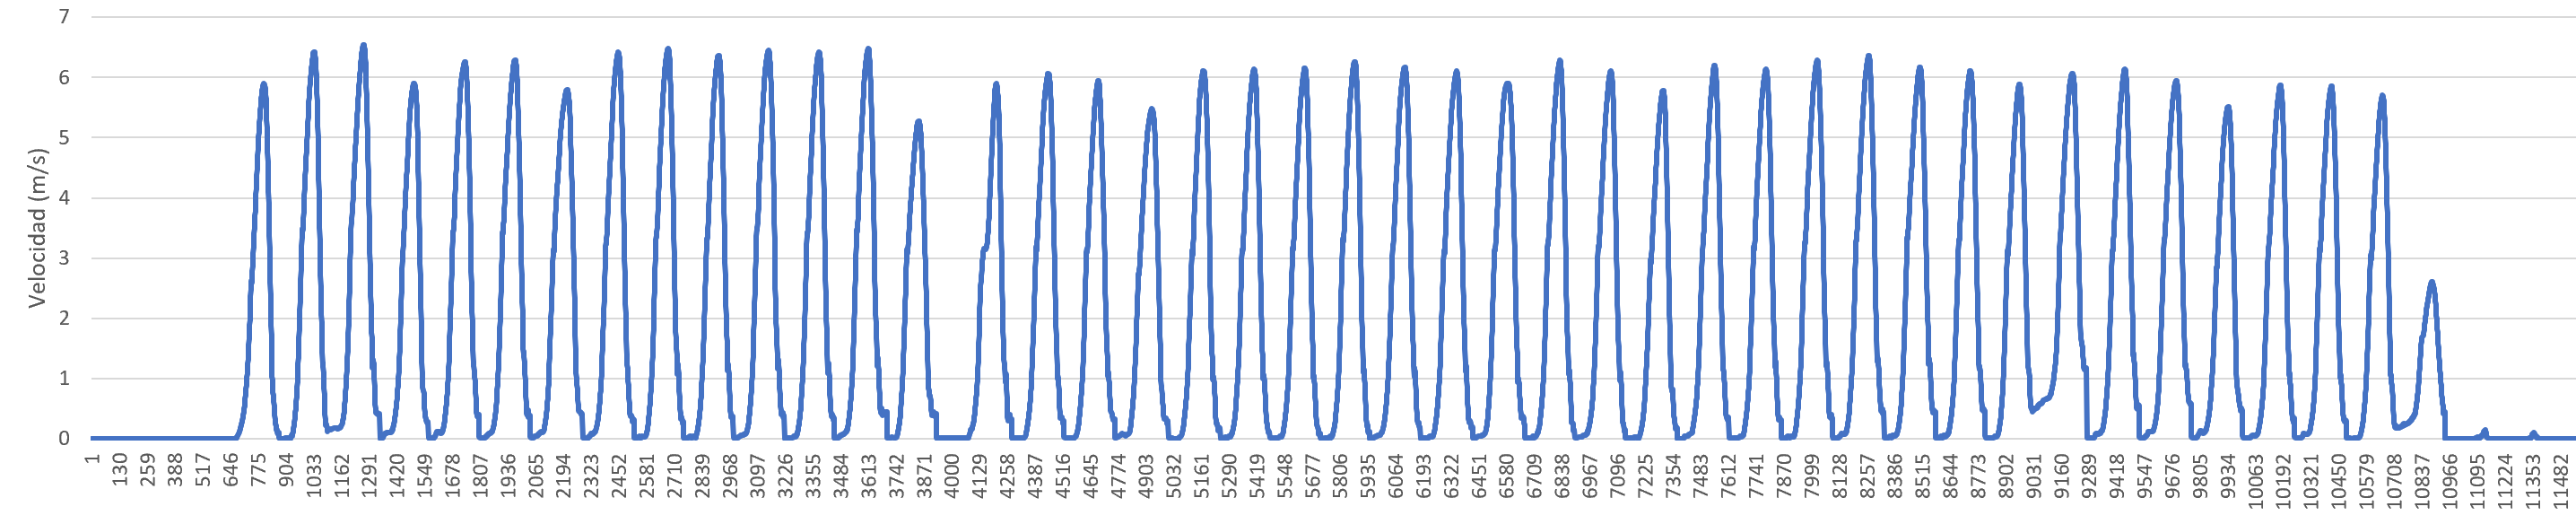
\includegraphics[clip,width=1.4 \columnwidth]{TESIS/imagenes/chap06/velocity-openshoe.PNG}
\caption{Velocidad del usuario calculada por el filtro de Kalman PARKIBIP, en $m/s$. Realizado con datos de prueba open source de Openshoe. La velocidad media lograda por PARKIBIP fue de 1.81$m/s$ versus el valor esperado 1.94 $m/s$. }
\label{fig:openshoe-velocity}
\end{figure}

Finalizando las comparaciones con los datos públicos de Openshoe, se presenta una gráfica de la trayectoria en las dimensiones x e y, en la unidad metros. La figura Fig. \ref{fig:openshoe-trajectory}, dibuja la la trayectoria recorrida por el sujeto en deambulación, iniciando en el posición $(x,y) =(0,0)$ dado por el punto naranja, y culminando en el punto $(x,y) =(-0.048,0.103)$. Lo que indica la cercanía respecto al valor esperado. 

\begin{figure}[h!]
\hspace*{-2.9cm}%
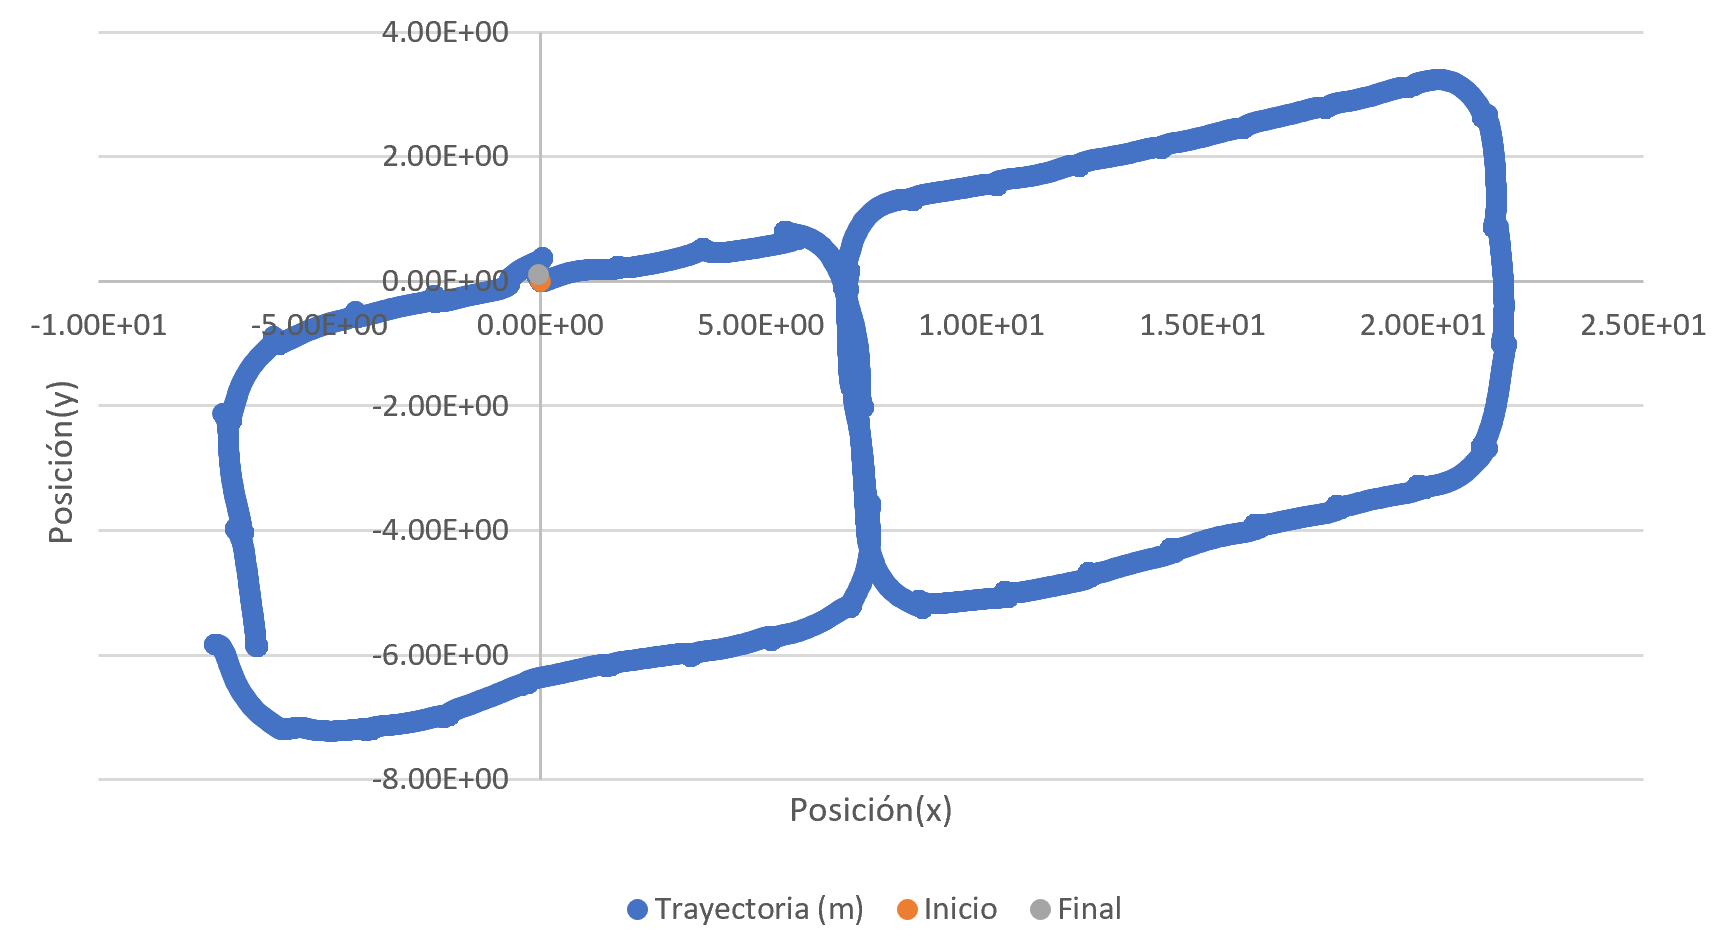
\includegraphics[clip,width=1.4 \columnwidth]{TESIS/imagenes/chap06/openshoe-trajectory.PNG}
\caption{Gráfico de la trayectoria en las dimensiones x e y, en en el sistema internacional de unidades -metros-. El sujeto inicia la marcha en la posición $(x,y) =(0,0)$ dado por el punto naranja, y culminando en el punto $(x,y) =(-0.048,0.103)$. Es decir, un ciclo cerrado.}
\label{fig:openshoe-trajectory}
\end{figure}

\section{Pruebas de PARKIBIP en lazo cerrado con referencias espacio-temporales }

En líneas generales, se realizan ciertas reflexiones respecto a la marcha de sujetos sin afecciones en la misma. Los participantes evaluados mediante pruebas experimentales fueron los mismos creadores del sistema y allegados; con una edad promedio de 28 años. Así, sobre la finalización del proyecto, se llevaron adelante 20 marchas aleatorias sobre una superficie plana que fueron registradas en una planilla Excel. La configuración establecida fue estimular al usuario de forma vibratoria y sonora según la regla seleccionada, para mejorar la calidad de la validación.

Primero, para cada marcha, se analizó la aceleración lineal instantánea y media del usuario -rotada al marco terrestre y extraída la gravedad-. Todas las aceleraciones registradas presentaron un patrón de comportamiento adecuado, siendo acotadas superiormente por una aceleración instantánea de 25 $m/s^2$ y con un movimiento cíclico compuesto por los períodos \textit{Stance} y \textit{Swing}. La aceleración promedio, contempladas todas las marchas, ascendió a 2.88 $m/s^2$, dentro de lo esperado.

En términos de estímulos, seleccionado el evento PARKIBIP \textit{onHeelStrike} -toque de talón-, para identificar el comienzo de la fase de \textit{Stance}, fueron contabilizados la cantidad de estímulos correspondientes a las pisadas. En general, los tres métodos detectores de velocidad cero presentaron resultados satisfactorios en la identificación de las fases de a marcha, con las siguientes particularidades:

\begin{itemize}
    \item \textit{Threshold}: En caso detectar momentos estacionarios, lo hace una única vez, mediante picos de aceleración. Si bien es un beneficio, ya que detecta adecuadamente el cambio de fase de la marcha, por otro lado no continúa el monitoreo del estado actual. Es decir, registra transiciones entre estados. Asimismo, el método es predispuesto a perder fases si el umbral es alto o a detectar mayores transiciones si el mismo es bajo.
    \item \textit{MV}: Presenta excelentes resultados en la detección de momentos estacionarios, mediante la supervisión continua del estado activo. Si bien el método desarrollado no falla en la estimación del estado \textit{stance}, en ocasiones presenta falsos-positivos, detectando un estado estacionario cuando en realidad estaba en movimiento. Por ende, emite unos pocos eventos incorrectos.   
    \item \textit{GLRT}: Similar a \textit{MV}, al incorporar el sensor giroscopio, GLRT ajusta las detecciones de los estados \textit{stance/swing}, logrando mejores resultados. Al ser preciso, mínimos movimientos angulares del tobillo del paciente generan transiciones de estados.
\end{itemize}

\noindent Luego, bajo el soporte de la funcionalidad que registra la duración de la sesión, la  Cadencia (i.e pasos por minutos) y la duración media del paso fueron calculadas apropiadamente, según el método y los eventuales falsos-positivos.  
\noindent Otra prueba realizada con éxito fue el evento PARKIBIP \textit{onFoG}. Esto es, transcurrido un intervalo de tres segundos en el que el pie se encontraba en una fase estacionaria, se  emitía un estimulo vibratorio/sonoro. En todas las ocasiones, el sistema actuó apropiadamente.

Además, se analizaron las velocidades instantáneas y medias de las marchas. Puesto que PARKIBIP no fue evaluado frente a otro sistema en tiempo real con el mismo sujeto, el parámetro espacio-temporal velocidad no fue validado con exactitud. Sin embargo, el sistema presentó valores de velocidad media acotados entre [0.57,1.92] $m/s$, siendo consistente con la velocidad de una marcha normal. A su vez, se probaron los reglas para estimular \textit{onInstantVelocityThreshold} y \textit{onAverageVelocityThreshold}. Ambas, cumplieron el objetivo de estimular al sujeto superado cierto umbral predefinido.

Para finalizar, cabe señalar que, aunque el parámetro espacio-temporal posición instantánea fue obtenido, el método que calcula la trayectoria no fue desarrollado. Esto se debió a la priorización de tareas, alcance del proyecto y tiempo disponible.